\documentclass[11pt]{article}

% ------------------------------------------------------------
% Packages
% ------------------------------------------------------------

\usepackage[margin=1in]{geometry}

\usepackage{amsmath}
\usepackage{amssymb}
\usepackage{amsthm}
\usepackage{mathtools}

\usepackage{graphicx}
\usepackage{booktabs}
\usepackage{multirow}
\usepackage{float}
\usepackage{subcaption}

\usepackage{algorithm}
\usepackage{algpseudocode}

\usepackage{hyperref}
\usepackage{cleveref}

\usepackage{natbib}

\usepackage{authblk}

% ------------------------------------------------------------
% Mathematical notation
% ------------------------------------------------------------

\newcommand{\AVaR}{\operatorname{AVaR}}
\newcommand{\VaR}{\operatorname{VaR}}
\newcommand{\EE}{\mathbb{E}}
\newcommand{\PP}{\mathbb{P}}
\newcommand{\RR}{\mathbb{R}}

\newcommand{\X}{\mathcal{X}}
\newcommand{\A}{\mathcal{A}}

% ------------------------------------------------------------
% Theorems
% ------------------------------------------------------------

\newtheorem{theorem}{Theorem}
\newtheorem{proposition}{Proposition}
\newtheorem{lemma}{Lemma}
\newtheorem{corollary}{Corollary}
\newtheorem{assumption}{Assumption}

% ------------------------------------------------------------
% Document
% ------------------------------------------------------------

\setlength\parindent{0pt}

\title{Decision-Aware Bellman Sampling for Static AVaR Control Using Gaussian Processes}

\author[1]{Dilzhan Zhangunissov}
\author[2]{Aruzhan Dauleshova}
\author[1]{Kerem U\u{g}urlu}

\affil[1]{Department of Mathematics, Nazarbayev University, Kazakhstan}
\affil[2]{Independent Researcher}

\date{\today}

\begin{document}
	
	\maketitle
	
	\begin{abstract}
We study finite-horizon Markov Decision Processes with continuous states, finite actions, and a static Average Value-at-Risk (AVaR) objective. The augmented-state formulation enables dynamic programming but introduces an additional continuous state variable, making exact solutions computationally expensive. We propose a probabilistic Approximate Dynamic Programming (ADP) method using Gaussian processes to approximate Q-functions in the difficult region of the augmented state space, while exploiting risk-neutral continuation elsewhere. Bellman backups are allocated using acquisition scores based on decision uncertainty, reachability, and tail relevance. We also derive approximation and policy-performance error bounds. Numerical experiments show that decision-aware sampling often achieves better policy performance per Bellman backup than random or uncertainty-based sampling. However, incorporating reachability or tail relevance does not consistently improve performance, and greater backup efficiency does not necessarily imply lower runtime. These results suggest that decision-aware Bellman allocation is a promising approach to computationally efficient risk-averse control.
\end{abstract}
	
	\section{Introduction}
\label{sec:introduction}

Traditional stochastic control often minimizes the expected cumulative cost. However, in applications where large losses are particularly meaningful, the expected cost may not adequately represent the risk of severe outcomes. Average Value-at-Risk (AVaR), also known as Conditional Value-at-Risk (CVaR) or Expected Shortfall (ES), provides an alternative by focusing on the upper tail of the cost distribution. The optimization representation of AVaR introduced by \cite{rockafellar-2002} makes it possible to formulate risk-averse control problems in terms of expected excess costs.

For Markov Decision Processes (MDPs), minimizing the static AVaR of cumulative cost is challenging because the objective does not directly admit standard Bellman recursion. \cite{bauerle-2011} addressed this problem using an augmented state that tracks the accumulated cost relative to a risk threshold. Although this formulation enables dynamic programming, it introduces an additional state dimension, making exact solutions computationally expensive for continuous-state problems.

Approximate Dynamic Programming (ADP) can reduce this computational cost, but its performance depends on how the available computational effort is allocated. In particular, approximating value functions accurately across the entire state space may be unnecessary when the main objective is to obtain a good policy. Approximation errors do not necessarily change the optimal action, as discussed through the action-gap phenomenon by \cite{farahmand-2011}. This motivates selecting Bellman updates according to their potential effect on policy decisions.

In this paper, we investigate a probabilistic ADP method based on Gaussian Processes (GPs) for finite-horizon static AVaR control. We exploit the risk-neutral structure of the augmented state space when the accumulated cost exceeds the threshold and use GP approximations in the remaining region. To allocate Bellman backups, we consider acquisition scores based on uncertainty about the optimal action, state reachability, and relevance to the AVaR tail. We also derive approximation and policy-performance error bounds, including the effects of the AVaR confidence level and outer threshold optimization.

We evaluate the method against exact dynamic programming, a baseline ADP algorithm, and alternative GP sampling strategies. The experiments show that decision-aware sampling often achieves better policy performance per Bellman backup than random or uncertainty sampling. However, adding reachability or tail weighting does not consistently improve the results, and backup efficiency does not necessarily imply lower runtime. These findings motivate further investigation of decision-aware allocation of computational effort in risk-averse control.
	
	\section{Related work}
\label{sec:related}

\subsection{AVaR control and approximate dynamic programming}
\label{rel:avar-mdp}

The optimization representation of AVaR introduced by \cite{rockafellar-2002} provides a foundation for risk-averse stochastic optimization. For Markov decision processes, applying AVaR to the cumulative cost generally prevents direct Bellman recursion on the original state space. \cite{bauerle-2011} addressed this problem by introducing an augmented state that tracks the remaining risk threshold. Their formulation also establishes the affine structure of the value function after the threshold has been crossed. Under nonnegative costs, this corresponds to the risk-neutral continuation used in this paper.

Several other approaches have been developed for risk-averse sequential decision making. \cite{chow-2015} proposed an augmented dynamic programming formulation based on the dual representation of AVaR, together with approximate value iteration. \cite{jiang-2018} studied risk-averse approximate dynamic programming with quantile-based risk measures and importance sampling. However, their recursively defined risk criteria differ from the static AVaR of cumulative cost considered here. More recently, \cite{muni-2026} developed an alternative Bellman formulation for static AVaR control based on reward redistribution.

These methods demonstrate that risk-averse control can be addressed through different dynamic programming formulations and approximation techniques. In the present work, we follow the augmented-state approach of B\"{a}uerle and Ott and exploit its established structural properties. Our focus is on approximating the remaining difficult region efficiently by allocating a limited number of Bellman backups to selected states.

\subsection{Gaussian processes and decision-aware sampling}
\label{rel:gp}

Gaussian processes have been widely used for value-function approximation in reinforcement learning. \cite{engel-2005} developed Gaussian-process methods for value and action-value estimation, while \cite{grande-2014} studied sample-efficient reinforcement learning using GPs. Unlike these approaches, our method uses GPs to approximate Q-functions from model-based Bellman targets in a backward finite-horizon recursion. The GP predictions provide both approximate Q-values and uncertainty estimates, which we use to guide the selection of Bellman updates.

Selective allocation of computational effort is also an established idea in approximate dynamic programming. \cite{wingate-2005} studied prioritization methods for Bellman updates, while \cite{ryzhov-2019} developed a Bayesian exploration framework for approximate dynamic programming. These methods show that computational resources can be allocated according to the expected usefulness of additional information. Our approach follows a similar principle but focuses specifically on uncertainty about the optimal action rather than value-function accuracy alone.

The motivation for decision-aware sampling is closely related to the action-gap phenomenon studied by \cite{farahmand-2011}, which explains why approximation errors do not necessarily change the optimal action. A related approach was developed by \cite{cakmak-2024}, who used Gaussian processes for contextual ranking and selection under a limited simulation budget. Our decision score follows the same general idea by measuring uncertainty in the ordering of the two actions with the lowest predicted Q-values. We adapt this criterion to select Bellman backups in the difficult region of an augmented static-AVaR MDP. We also investigate reachability and tail relevance, which are related to importance sampling in risk-averse ADP \citep{jiang-2018} and tail-focused sampling for AVaR evaluation \citep{bourigault-2026}.
	
	\section{Problem formulation}
\label{sec:problem}

\subsection{Finite-horizon Markov decision process}
\label{problem:mdp}

Consider a finite-horizon controlled Markov process with time
indices $t=0,1,\ldots,T$, continuous state space
$\X\subseteq\RR$, and finite action space
$\A$. The system's dynamics are
\begin{equation}
	x_{t+1} = f(x_t, a_t, \xi_t)
	\label{transition-dynamics}	
\end{equation}
where 
\begin{itemize}
	\item $x_t\in\X$ denotes the state at time $t$,
	\item $a_t\in\A$ is the selected action, and
	\item $\{\xi_t\}_{t=0}^{T-1}$ is a sequence of independent and identically distributed random disturbances.
\end{itemize}
The initial state $x_0\in\X$ is assumed to be fixed.

Let the cumulative cost induced by a policy $\pi$ be defined as
\begin{equation}
	C^\pi = \sum_{t=0}^{T-1}c_t(x_t,a_t)+c_T(x_T),
	\label{total-cost}
\end{equation}
where 
\begin{itemize}
	\item $c_t:\X \times \A \to\RR_{\geq 0}$ is the stage cost at time $t$, and
	\item $c_T:\X\to\RR_{\geq 0}$ is the terminal cost, depending only on the terminal state.
\end{itemize} 

We assume that the dynamics and cost functions are measurable
and that the cumulative cost is integrable under every
admissible policy.

\subsection{AVaR objective}
\label{problem:avar}

For confidence level $\alpha\in(0,1)$, the objective is
\begin{equation}
	\min_{\pi} \AVaR_{\alpha}(C^\pi).
	\notag
	\label{minimize-avar}
\end{equation}

Using the \cite{rockafellar-2002} representation,
\begin{equation}
	\AVaR_{\alpha}(X) = \min_{\eta\in\RR} \left[ \eta + \frac{1}{1-\alpha} \EE\left[(X-\eta)_+\right] \right].
	\label{ru-objective}
\end{equation}

Hence the control problem can be written as
\begin{equation}
	\begin{array}{rl}
		\displaystyle \min_{\pi} \AVaR_{\alpha} (C^{\pi}) &= \displaystyle \min_{\pi} \min_{\eta \in \RR} \left[ \eta + \frac{1}{1 - \alpha} \EE [(C^{\pi} - \eta)_+] \right] \\
		&= \displaystyle \min_{\eta \in \RR} \left\{ \eta + \frac{1}{1 - \alpha} \min_{\pi} \EE [(C^{\pi} - \eta)_+] \right\}
	\end{array}
	\label{avar-objective}
\end{equation}

Since the ramp function acts on the cumulative cost, the problem generally cannot be solved using standard Bellman recursion on the original state space.

\subsection{Augmented-state formulation}
\label{problem:augmentation}

To make dynamic programming tractable, we introduce an augmented state, according to \cite{bauerle-2011}:
\begin{equation}
	y_t = \sum_{s=0}^{t-1} c_s(x_s, a_s) - \eta,
	\label{augmented-state-sum}
\end{equation}
or, equivalently,
\begin{equation}
	y_{t+1} = y_t + c_t(x_t, a_t), \quad y_0 = -\eta
	\label{augmented-state-recursive}
\end{equation}

The terminal value function then becomes
\begin{equation}
	V_T(x, y) = (y + c_T(x))_+.
	\label{value-function-terminal}
\end{equation}

For $t<T$, we can define
\begin{equation}
	Q_t(x, y, a) = \EE \left[ V_{t+1} \left( x_{t+1}, y_{t+1} \right) \mid x_t = x, y_t = y, a_t = a \right]
	\label{q-function}
\end{equation}

and
\begin{equation}
	V_t(x, y) = \min_{a \in \A} Q_t(x, y, a).
	\label{value-function}
\end{equation}

The optimal fixed-$\eta$ value for the entire horizon is therefore
\begin{equation}
	V_0(x_0,-\eta).
	\label{root-value}
\end{equation}

The corresponding complete AVaR objective is
\begin{equation}
	J(\eta) = \eta + \frac{1}{1-\alpha} V_0(x_0,-\eta),
	\label{root-avar}
\end{equation}
and
\begin{equation}
	\eta^\star \in \arg\min_{\eta} J(\eta).
	\notag
	\label{optimal-eta}
\end{equation}

\subsection{Risk-neutral region of the augmented state space}
\label{problem:rn-region}

Once $y_t \geq 0$ at some time step $t$, under nonnegative stage and terminal costs,
\begin{equation}
	y_s = \underbrace{y_t}_{\geq 0} + \sum_{u=t}^{s-1} \underbrace{c_u(x_u, a_u)}_{\geq 0}, \quad t < s \leq T
	\notag
	\label{positive-augmented}
\end{equation}

Thus, the ramp function $(\cdot)_+$ does not change the objective of the optimization, meaning that
\begin{equation}
	Q_t(x, y, a) = y + Q_t^{\text{RN}}(x, a),
	\label{q-func-using-rn}
\end{equation}
and the optimal action remains identical
\begin{equation}
	\arg\min_{a \in \A} Q_t(x, y, a) = \arg\min_{a \in \A} Q_t^{\text{RN}}(x, a),
	\label{q-func-rn-argmin}
\end{equation}
where $Q_t^{\text{RN}}$ is a risk-neutral Q-function corresponding to the following control optimization problem
\begin{equation}
	Q_t^{\text{RN}}(x, a) = c_t(x, a) + \EE \left[ V_{t+1}^{\text{RN}} (x_{t+1}) \mid x_t = x, a_t = a \right],
	\label{q-rn-bellman}
\end{equation}
and
\begin{equation}
	V_t^{\text{RN}}(x) = \min_{a \in \A} Q_t^{\text{RN}}(x, a), \quad V_T^{\text{RN}}(x) = c_T(x).
	\label{value-rn}
\end{equation}

\subsection{Risk-neutral Q-function approximation}
\label{problem:rn-approximation}

We approximate the risk-neutral Q-function using backward dynamic programming with regression. Starting from the terminal condition
\begin{equation}
	V_T^{\text{RN}}(x)=c_T(x),
	\notag
	\label{value-rn-terminal}
\end{equation}

the Q-function and its approximation at $t=T-1$ are given by
\begin{equation}
	\hat{Q}_{T-1}^{\text{RN}} \approx Q_{T-1}^{\text{RN}}(x,a) = c_{T-1}(x,a) + \EE \left[c_T(x_T) \mid x_{T-1} = x,a_{T-1} = a\right].
	\notag
	\label{q-rn-preterminal}
\end{equation}

The corresponding value function approximation is
\begin{equation}
	\hat V_{T-1}^{\text{RN}}(x) = \min_{a \in \A}\hat Q_{T-1}^{\text{RN}}(x,a).
	\notag
	\label{value-rn-preterminal}
\end{equation}

This approximation is then used to construct the Bellman targets at the preceding time step,
\begin{equation}
	\hat Q_t^{\text{RN}}(x,a) \approx c_t(x,a) + \EE \left[ \hat V_{t+1}^{\text{RN}}(x_{t+1}) \mid x_t=x,a_t=a \right],
	\label{q-rn-approx-bellman}
\end{equation}
\begin{equation}
	\hat{V}_t^{\text{RN}}(x) = \min_{a \in \A} \hat{Q}_t^{\text{RN}}(x, a).
	\notag
	\label{value-approx-bellman}
\end{equation}

The procedure is repeated backward from $t=T-1$ to $t=0$.

\subsection{Computational challenge}
\label{problem:challenge}

The state augmentation allows us to use dynamic programming, making the problem tractable. However, the problem is now formulated over $\X \times \RR$, leaving us with two continuous states to handle. This makes the direct Bellman solution very expensive, especially as horizon and discretization increase.

The risk-neutral region $y \geq 0$ reduces this difficulty by allowing us to use risk-neutral continuation approximations. The remaining $y < 0$ region still requires the calculation (or approximation) of the augmented-state value function.

Under a limited computational budget, evaluating the Bellman operator uniformly across this region may be inefficient as different states have different effects on policy and resulting AVaR objective. This motivates the development of a sampling strategy that allocates Bellman evaluations to states where they are most relevant to the accuracy of the solution.
	
	\section{Methodology}
\label{sec:method}

\subsection{Exact dynamic programming}
\label{method:exact}
Both the proposed and baseline algorithms can be verified against an exact dynamic programming solution if the horizon $T$ is small. The expectation in \eqref{q-function} is computed using Riemann summation
\begin{equation}
	\begin{array}{rl}
		\EE \left[ V_{t+1} (x_{t+1}, y_{t+1}) \mid x_t = x, y_t = y, a_t = a \right] & \displaystyle = \int V_{t+1} (x_{t+1}, y_{t+1}) p_{x_{t+1}} \left( x_{t+1} \mid x_t = x, a_t = a \right) d x_{t+1} \\
		& \displaystyle = \int V_{t+1} (f(x_t, a_t, \xi_t), y_t + c_t(x_t, a_t))\ p_{\xi}(\xi_t)\ d \xi_t \\
		& \displaystyle \approx \sum_{i=0}^{N_{\xi}} V_{t+1} (f(x_t, a_t, \xi^{(i)}), y_t + c_t(x_t, a_t))\ w_i
	\end{array}
	\label{riemann-expectation}
\end{equation}
where
\begin{itemize}
	\item $p_{\xi}$ is the density of disturbance distribution,
	\item $\xi^{(i)}$ are discretization points of the disturbance domain, defined by:
	\begin{itemize}
		\item $\xi^{(0)} = \xi_{\text{min}},$
		\item $\xi^{(N_{\xi})} = \xi_{\text{max}},$
		\item $\xi^{(i+1)} = \xi^{(i)} + \Delta_{\xi},$ 
		\item $\Delta_{\xi} = \frac{\xi_{\text{max}} - \xi_{\text{min}}}{N_{\xi}},$
	\end{itemize}
	\item $w_i = \frac{p_{\xi}(\xi^{(i)})}{\sum_j p_{\xi}(\xi^{(j)})}$ is the normalized discrete weights of points.
\end{itemize}

For a sufficiently wide integration domain and fine discretization mesh, the numerical approximation is expected to approach the true expectation. In this paper we refer to this method as \textit{Exact Dynamic Programming} to distinguish it from the approximate dynamic programming methods introduced in the following subsections. Here, \textit{exact} means that the Bellman recursion is solved directly, without approximating the value functions.

\subsection{Baseline approximate dynamic programming}
\label{method:baseline-adp}

The exact dynamic programming algorithm serves as a reliable reference for small horizons, but its computational cost can grow exponentially with the horizon. To reduce computational cost, we use an Approximate Dynamic Programming (ADP) algorithm.

The method is based on Monte Carlo rollouts. To initialize the value function at an unseen state $(t,x,y)$, we simulate $N$ trajectories from that state. The actions in the trajectories are chosen using the approximate risk-neutral policy, which provides a computationally cheap way to estimate the remaining cumulative cost. For each trajectory, we calculate the remaining cumulative cost and apply the ramp function. The initial estimate is then obtained by averaging these values.

To improve the estimate, we also use the risk-neutral value approximation and define
\begin{equation}
	\hat{V}_t^{\text{init}}(x,y) = \max\left\{
	\frac{1}{N}\sum_{i=1}^N (y+C_{t:T}^{(i)})_+,\ 
	\left(y+\hat{V}_t^{\text{RN}}(x)\right)_+
	\right\},
	\label{value-initializer}
\end{equation}
where $C_{t:T}^{(i)}$ is the remaining cumulative cost of the $i$-th trajectory.

In the equation above we have used Jensen's bound: given that the ramp function is convex, we can obtain
\begin{equation}
	\begin{array}{rl}
		V_t(x, y) & \displaystyle = \min_{\pi} \EE^{\pi} \left[ \left( y + C_{t:T}^{\pi} \right)_+ \right] \\
		& \displaystyle \geq \min_{\pi} \left( \EE^{\pi} \left[ y + C_{t:T}^{\pi} \right] \right)_+ \\
		& = \left( y + V_t^{\text{RN}} (x) \right)_+
	\end{array}
	\notag
	\label{value-jensen}
\end{equation}
Since the approximation of the risk-neutral value function is used we cannot guarantee that the right-hand side is a valid lower bound. However, using the risk-neutral approximation gave us a useful proxy to a lower bound for the current value function. Monte Carlo estimation was compared to the risk-neutral value function and their maximum was used as the initial value.

At terminal states, we use the exact terminal value. For visited nonterminal states, we apply the Bellman updates described in Section~\ref{problem:augmentation}, using the initialized values whenever necessary. The initialized values are stored and reused to avoid repeated simulations.

For $y \geq 0$, we can use approximation of the risk-neutral Q-function as discussed in Section~ \ref{problem:rn-approximation}. In this paper we use linear regression to approximate each Q-function:
\begin{equation}
	\hat{Q}_t^{\text{RN}}(x, a) = \phi^T(x) \theta_{t, a} \approx Q_t^{\text{RN}}(x, a)
	\label{linear-q-approx}
\end{equation}
where 
\begin{itemize}
	\item $\phi(x): \X \to \mathbb{R}^{d}$ is a feature map,
	\item $\theta_{t, a} \in \mathbb{R}^{d}$ is a vector of regression parameters.
\end{itemize}
The feature map combines quadratic and radial basis function (RBF)
features:
\begin{equation}
	\phi(x) =
	\begin{bmatrix}
		1 & z & z^2 & \psi_1(x) & \cdots & \psi_{d-3}(x)
	\end{bmatrix}^{\top},
	\label{feature-map}
\end{equation}
where $z \in [-1,1]$ is obtained by linearly scaling $x$, and
\begin{equation}
	\psi_i(x) = \exp\left(-\frac{(x-c_i)^2}{2\ell^2}\right), \quad i=1,\ldots,d-3.
	\notag
	\label{rbf}
\end{equation}
The RBF centers $c_i$ are uniformly spaced over a slightly enlarged interval around $[x_{\min},x_{\max}]$.

The model training process is recursive as described in Section~\ref{problem:rn-approximation}. 

To reuse previously computed values, we store them in a lookup table. Since the state variables $x$ and $y$ are continuous, we round them to six decimal places before constructing the cache keys. This allows sufficiently close states to share the same stored value, reducing the number of repeated computations at the cost of a small additional approximation.

The full algorithm can be found in Appendix~\ref{app:baseline-adp}.

The baseline ADP reduces computational cost by exploiting the risk-neutral region, reusing previously computed values, and approximating the values of unseen states using Monte Carlo rollouts instead of full Bellman recursion. However, its accuracy depends on which states are visited during training, and the algorithm does not explicitly account for the importance of individual Bellman updates.

\subsection{Proposed probabilistic ADP}
\label{method:prob}

The baseline ADP reduces computational cost, but it does not explicitly account for the importance of states when performing Bellman updates. As discussed in Section~\ref{problem:challenge}, different states may have different effects on the resulting policy and AVaR objective. To address this, we propose a probabilistic ADP method that allocates Bellman evaluations to selected states in the region $y<0$, while continuing to use the risk-neutral approximation for $y\geq 0$.

The proposed algorithm uses Gaussian Processes (GPs) to approximate the Q-functions, providing both point predictions of the value and estimates of uncertainty. To decide where to perform Bellman updates, we construct sets of candidate states and evaluate them using three criteria: reachability, uncertainty about the optimal action, and relevance to the AVaR tail. These criteria guide the allocation of a limited computational budget. The GP models are then trained backward in time using the selected Bellman evaluations. Additionally, the use of GPs reduces our need to discretize the state space as we have done in the baseline ADP by rounding the states. The following subsections describe each component of the proposed method. The resulting algorithm can be found in Appendix~\ref{app:prob-adp}.

\subsubsection{GP approximation of Q-functions}
\label{method:gp-approx}

For the region $y<0$, we approximate the Q-functions using GPs. Unlike the regression models used for the risk-neutral approximation, GPs provide both point predictions and estimates of uncertainty. We train a separate GP model for each time step $t$ and action $a \in \A$, using the augmented state $s = (x,y)$ as input.

The training data are obtained by applying the Bellman operator at selected augmented states. For a training state $s_j=(x_j,y_j)$ and action $a$, the target value is calculated as
\begin{equation}
	q_{t,a}^{(j)}
	=
	\sum_{\xi^{(i)}\in\Xi} w_i
	\hat{V}_{t+1}\left(
	f(x_j,a,\xi^{(i)}),
	y_j+c_t(x_j,a)
	\right).
	\label{gp-bellman-target}
\end{equation}
where $\hat{V}_{t+1}$ is the value function approximation obtained at the next time step. The resulting training dataset for each GP is
\begin{equation}
	\mathcal{D}_{t, a} = \left\{ \left( s_j, q_{t, a}^{(j)} \right) \right\}_{j=1}^{n_t}
	\notag
	\label{gp-training-dataset}
\end{equation}
where $n_t$ is the number of selected training states at time $t$.


We fit a GP with mean function $m_{t,a}$ and covariance kernel $k_{t,a}$ to the approximate Bellman targets defined in \eqref{gp-bellman-target}.

We use an RBF kernel with fixed hyperparameters and scale the GP inputs using fixed state-space bounds. Before fitting each GP, the training targets are standardized, and predictions are transformed back to their original scale.

Given the training data, the GP provides a predictive mean $\mu_{t,a}(s)$ and variance $\sigma_{t,a}^2(s)$. These are calculated as
\begin{equation}
	\begin{array}{c}
		\mu_{t, a}(s) = m_{t, a}(s) + k(s)^{\top} (K + \lambda I)^{-1} (q_{t, a} - m_{t, a}), \\
		\sigma_{t, a}^{2} (s) = k_{t, a}(s, s) - k(s)^{\top} (K + \lambda I)^{-1} k(s),
	\end{array}
	\label{gp-inference}
\end{equation}
where:
\begin{itemize}
	\item $K$ is the covariance matrix of the training inputs,
	\item $k(s)$ is the vector of covariance between training inputs and $s$,
	\item $q_{t, a}$ is the vector of training targets,
	\item $m_{t, a}$ is the prior mean at training inputs,
	\item $\lambda$ is a regularizer.
\end{itemize}

We use the predictive mean to approximate the Q-functions:
\begin{equation}
	\hat{Q}_t(x, y, a) = \mu_{t, a}(x, y),
	\label{gp-predictive-mean}
\end{equation}
which gives the corresponding value function and policy:
\begin{equation}
	\begin{array}{c}
		\displaystyle \hat{V}_t(x, y) = \max \left\{ \min_{a \in \A} \hat{Q}_t (x, y, a),\ \left( y + \hat{V}_t^{\text{RN}}(x) \right)_+ \right\},\\
		\displaystyle \hat{\pi}_t(x, y) = \arg\min_{a \in \A} \hat{Q}_t(x, y, a).
	\end{array}
	\label{gp-value-policy}
\end{equation}

These approximations are used only for $y<0$. For $y\geq0$, we continue using the risk-neutral approximation described earlier, while at $t=T$ we use the exact terminal value.

The predictive uncertainty $\sigma_{t,a}(x,y)$ provides information about how uncertain the GP model is at a particular state. It measures uncertainty within the fitted model, but it does not necessarily represent the actual Q-function approximation error. We use this information when selecting states for Bellman updates, as described in the following subsections.

\subsubsection{Candidate-state construction}
\label{method:candidate}

Since the augmented state space $\X \times \RR$ is continuous, we cannot evaluate the Bellman operator at every possible state. Instead, for each time step $t$, we construct a finite set of candidate states

\begin{equation}
	\mathcal{S}_t = \{s_t^{(j)}\}_{j=1}^{M_t},
	\qquad s_t^{(j)}=(x_t^{(j)},y_t^{(j)}),
	\label{candidate-set}
\end{equation}
where $M_t$ is the number of candidates at time $t$. These states are used to select the points at which Bellman updates will be performed.

The candidate states are restricted to the region $y<0$, since for the region $y\geq0$ we use risk-neutral approximation. Note that, since the stage costs are nonnegative, the augmented state satisfies $y_t\geq-\eta$ for a fixed threshold $\eta$.

To construct the candidate set, we consider a range of possible values of $x$ at each time step, based on the system dynamics and disturbance distribution. We then generate candidate states from the region
\begin{equation}
	\begin{array}{lr}
	\mathcal{R}_t =
	[x_t^{\text{min}},x_t^{\text{max}}]\times[-\eta,0), & 0 < t < T \\
	\mathcal{R}_t = \{ (x_0, -\eta) \}, & t=0,
	\end{array}
	\label{candidate-region}
\end{equation}
where $x_t^{\text{min}}$ and $x_t^{\text{max}}$ define the range of states considered at time $t$. We then select candidate states from this region without discretizing the entire state space.

However, not every state in this region is necessarily reachable. Since $y$ depends on $x$ as it accumulates the costs through the trajectory, some candidate states might be unlikely.

To avoid performing Bellman updates at all candidate states, we apply a scoring system to determine which candidate states should receive more computational effort. The acquisition scores are described in the following subsection.

\subsubsection{Bellman acquisition scores}
\label{method:acquisition}

The candidate set $\mathcal S_t$ contains possible states for Bellman updates. However, evaluating the Bellman operator at every candidate would be computationally expensive. To select the most useful states, we introduce acquisition scores based on three criteria: uncertainty about the optimal action, reachability, and relevance to the AVaR tail.

\paragraph{Decision uncertainty.}

The first criterion measures how uncertain the GP models are about the optimal action. Since our objective is to obtain an accurate policy, reducing uncertainty about the optimal action may be more important than reducing the approximation error of every Q-function.

For a candidate state $s=(x,y)$, let $a_1$ and $a_2$ denote the actions with the smallest and second-smallest GP predictive means, respectively. We define the predicted action gap as

\begin{equation}
	\Delta_t(s)
	=
	\mu_{t,a_2}(s)-\mu_{t,a_1}(s).
	\label{decision-gap}
\end{equation}

A small gap indicates that the two actions have similar predicted values. However, the gap alone does not tell us how confident the GP models are about their ordering.

The GP predictions are Gaussian. Assuming that the GP predictions for different actions are independent, their difference is also Gaussian. Using this fact we can estimate the probability of the second action being better than the first one. Let us first define their difference as a Gaussian
\begin{equation}
	\begin{array}{rl}
		Q_1 & \sim \mathcal{N}(\mu_{t, a_1}(s), \sigma_{t, a_1}^2(s)) \\
		Q_2 & \sim \mathcal{N}(\mu_{t, a_2}(s), \sigma_{t, a_2}^2(s)) \\
		Z_t(s) & = Q_2 - Q_1 \\
		& \sim \mathcal{N}(\Delta_t(s), \sigma_{t, a_1}^2(s) + \sigma_{t, a_2}^2(s))
	\end{array}
	\notag
	\label{action-difference-distribution}
\end{equation}
Now we can define a decision score as
\begin{equation}
	\begin{array}{rl}
		D_t(s) &= 2 \PP \left( Z_t(s) < 0 \right) \\
		& \displaystyle = 2 \Phi \left( -\frac{\Delta_t(s)}{\sqrt{\sigma_{t, a_1}^2(s) + \sigma_{t, a_2}^2(s)}} \right)
	\end{array}
	\label{decision-score}
\end{equation}
where $\Phi$ is the standard normal cumulative distribution function (CDF). The factor of 2 normalizes the score to the range $[0,1]$.

Larger values of $D_t(s)$ show greater uncertainty about the ordering of the two actions. This score is a proxy for decision uncertainty rather than the exact probability of selecting the wrong action, since other actions are not considered in the comparison.

We also define an uncertainty score
\begin{equation}
	U_t(s) = \max_{a \in \A} \sigma_{t, a}(s)
	\label{uncertainty-score}
\end{equation}
which measures the largest predictive standard deviation among the Q-function GP models, regardless of their predicted values.

\paragraph{Reachability.}

The second criterion measures how close a candidate state is to states visited during simulated trajectories. Bellman updates at states that are unlikely to be visited may have little effect on the resulting policy.

To estimate reachability, we simulate trajectories under a selected policy and collect the visited states at each time step. For each candidate $s$, we then find its $k$ nearest neighbors among the rollout states.

Since $x$ and $y$ can have different scales and are correlated, we use the Mahalanobis distance:

\begin{equation}
	d_t(s,s')
	=
	\sqrt{
		(s-s')^T
		(\Sigma_t+\varepsilon I)^{-1}
		(s-s')
	},
	\label{mahalanobis-distance}
\end{equation}
where $\Sigma_t$ is the covariance matrix of the rollout states at time $t$, and $\varepsilon>0$ is a small regularization parameter.

We then define a reachability score $R_t(s)$ using a distance from a state $s$ to its k-th nearest neighbor $\tilde{s}^{(k)}$:
\begin{equation}
	R_t(s) = \frac{1}{d_t(s, \tilde{s}^{(k)})^2 + \delta}
	\label{reachability-score}
\end{equation}
with $\delta > 0$ being a constant that prevents division by zero. The scores are then normalized to the range $[0, 1]$ by dividing each over the maximal score across the candidate states.

This is not the only way to define reachability. One can also consider average distances to nearest neighbors, state visitation probabilities or densities, or other measures of reachability.

\paragraph{Tail relevance.}

AVaR depends on the tail of the total cost distribution, so we want to give more attention to the states that are more relevant to the distribution tail.

Recall that the terminal value function is
\begin{equation}
	V_T(x,y)=(y+c_T(x))_+.
	\notag
\end{equation}

Therefore, a trajectory contributes a positive value to the fixed-$\eta$ objective only when its total cost exceeds $\eta$. Thus, the score measures relevance to costs exceeding the chosen threshold $\eta$, which may differ from the actual AVaR tail.

Using simulated trajectories, we can estimate the tail relevance of a candidate state from the outcomes of nearby rollout states. One possible score is

\begin{equation}
	L_t(s)
	=
	\frac{1}{k}
	\sum_{i\in\mathcal N_k(s)}
	\mathbb{I}
	\left\{
	y_T^{(i)}+c_T(x_T^{(i)})>0
	\right\},
	\label{tail-score}
\end{equation}

where $\mathcal N_k(s)$ now denotes the indices of the nearest rollout states, and $(x_T^{(i)},y_T^{(i)})$ is the terminal state of the corresponding trajectory.

This score estimates how frequently trajectories passing near a candidate end up in the AVaR tail. It is based on the rollout policy and does not necessarily represent the tail probability under the optimal policy.

\paragraph{Combination of acquisition scores.}

The described criteria provide different information about the usefulness of a Bellman update. Decision uncertainty identifies states where the optimal action is unclear, reachability favors states that are likely to be visited, and tail relevance favors states associated with larger cumulative costs.

We can use these scores separately or combine them into a single acquisition function:
\begin{equation}
	A_t(s)
	=
	F\left(D_t(s),R_t(s),L_t(s)\right),
	\label{acquisition-score-general}
\end{equation}
where $F$ denotes the selected combination rule. Different constructions of $A_t(s)$ result in different policies, giving us a field to experiment on.

\subsubsection{Backward training algorithm}
\label{method:training}

We train the GP models backward in time, starting from $t=T-1$ and continuing to $t=1$. The exact terminal value function is used to calculate the Bellman targets at $t=T-1$.

For acquisition methods involving reachability or tail relevance, we first simulate trajectories under the approximate risk-neutral policy. The visited states and terminal costs are then used to calculate the corresponding acquisition scores.

At each time step, we randomly select $N_{\text{init}}$ states from the candidate set $\mathcal{S}_t$. For each selected state, we calculate the Bellman targets for all actions and fit the initial GP models.

We then calculate acquisition scores for the remaining candidate states using the fitted GP models. The states with the highest scores are selected in batches. After each batch, we calculate the new Bellman targets, add them to the training data, and refit the GP models. This continues until the computational budget for the current time step is reached. For random sampling, all training states are selected randomly and the GP models are fitted only once.

The Bellman targets are calculated using the value-function approximation at the next time step. For $y<0$, we use the GP prediction together with the risk-neutral approximation and the lower bound of zero. For $y\geq 0$, we use the risk-neutral continuation, while at $t=T$ we use the exact terminal value.

After training the GP models for $t=1,\ldots,T-1$, we calculate the Q-values at the initial state $(x_0,-\eta)$ directly using the Bellman operator. Therefore, no GP model is needed at $t=0$. The resulting value is then used in the outer optimization over $\eta$, discussed in the following subsection.

\subsection{Outer optimization over $\eta$}
\label{method:outer-optimization}

Recall the optimization problem \eqref{avar-objective}:
\begin{equation*}
	\displaystyle \min_{\pi} \AVaR_{\alpha}(C^{\pi}) = \min_{\eta \in \RR} \left\{ \eta + \frac{1}{1 - \alpha} \min_{\pi} \EE [(C^{\pi} - \eta)_+] \right\}
\end{equation*}

In the previous subsections we have formulated baseline ADP and probabilistic ADP methods to solve the inner optimization problem for fixed $\eta$. In this subsection we will discuss the outer optimization problem over the threshold $\eta$. Consider a finite set of candidate thresholds
\begin{equation}
	\mathcal{H} = \left\{ \eta_1, \eta_2, \dots, \eta_{N_{\eta}} \right\}
	\notag
	\label{eta-family}
\end{equation}
over which to search for an optimal threshold.

Then, we modify the candidate domain stated in \eqref{candidate-region} as
\begin{equation}
	\mathcal{R}_t = [x_t^{\min},x_t^{\max}] \times[-\max\mathcal{H}, 0), \quad 0<t<T.
	\label{candidate-set-multiple-eta}
\end{equation}

This allows the same GP models to be used for
all candidate thresholds.


\paragraph{Baseline ADP}

While we cannot modify the baseline ADP solution to account for several values of $\eta$ at the same time, we can use a shared cache $\mathcal{C}$ to reuse the already calculated value functions. After calculating all of the values $\hat{V}_0(x_0, -\eta)$ for $\eta \in \mathcal{H}$ we can define the optimal approximate $\eta$ as
\begin{equation}
	\hat{\eta} = \arg\min_{\eta in \mathcal{H}} \hat{J}(\eta) = \arg\min_{\eta \in \mathcal{H}} \left\{ \eta + \frac{1}{1-\alpha} \hat{V}_0(x_0, -\eta) \right\}.
	\label{optimal-eta-baseline}
\end{equation}

\paragraph{Probabilistic ADP}

For probabilistic ADP, we can avoid training separate GP models for each $\eta \in \mathcal{H}$. Instead, we train a single collection of GP models for $t=1,\ldots,T-1$, using candidate states that cover the relevant range of augmented states for all thresholds in $\mathcal{H}$. We then evaluate the Bellman operator at $(x_0,-\eta)$ for each candidate threshold, without training a GP model at $t=0$. The resulting values $\hat{V}_0(x_0,-\eta)$ are used to calculate the corresponding objectives $\hat{J}(\eta)$ and select the best threshold. Each evaluation at the initial state requires one Bellman backup per action and is included in the computational budget.

The reuse of the training GPs is possible because the threshold enters the augmented problem only through the initial condition $y_0=-\eta$. The Bellman recursion at a given augmented state does not otherwise depend on $\eta$. The fitted continuation models can therefore be shared across root queries, provided that their training domain covers the required augmented states.

To conclude the section, we have stated an exact dynamic programming solution to compare the approximate methods against. The exact DP algorithm estimates the expectation using Riemann summation. It is computationally expensive, but can serve as a reliable benchmark for the approximate algorithm. The baseline ADP algorithm was designed using Monte Carlo rollouts and value initialization at unseen states. The main focus of the section is the proposed probabilistic ADP algorithm, which performs Q-function approximation using Gaussian processes and allocates Bellman backups to the candidate states using scoring based on decision uncertainty, reachability, and tail relevance of the candidates. At the end of the section we have briefly discussed an outer optimization over the threshold $\eta$ for baseline and probabilistic ADP algorithms.
	
	\section{Theoretical analysis}
\label{sec:theory}
 
\subsection{Preliminaries and assumptions}
\label{theory:preliminaries}

We consider the finite-horizon MDP and its augmented-state
formulation introduced in Section~\ref{sec:problem}.
Throughout this section, $V_t$ and $\hat{V}_t$ denote the
exact and approximate augmented-state value functions,
respectively. Similarly, $V_t^{\text{RN}}$ and
$\hat{V}_t^{\text{RN}}$ denote their risk-neutral counterparts.

The exact value and Q-functions are defined with respect
to the original continuous disturbance distribution.
The local approximation errors also account for numerical
integration errors introduced by the algorithms.

We make the following assumptions:
\begin{enumerate}
	\item \textbf{Nonnegative costs.}
	The stage and terminal costs are nonnegative
	\begin{equation*}
		c_t(x,a) \geq 0, \qquad c_T(x) \geq 0.
	\end{equation*}
	
	\item \textbf{Well-defined values.}
	All expectations appearing in the Bellman equations
	are finite on the states considered in the analysis.
	
	\item \textbf{Threshold domain.}
	The outer optimization is restricted to a compact
	interval $\mathcal{I}_\eta \subset \mathbb R$,
	assumed to contain at least one global optimal threshold
	$\eta^*$. The numerical optimization uses a
	finite candidate set $\mathcal{H} \subset \mathcal{I}_\eta$.
\end{enumerate}

For each $t$, let $\mathcal{Z}_t$ denote the set of augmented states $(x,y)$ reachable from $(x_0,-\eta)$, with $\eta\in\mathcal{I}_{\eta}$, under admissible action sequences and noise realizations.

We partition this domain into
\begin{equation}
	\mathcal{Z}_t^+ = \{ (x, y) \in \mathcal{Z}_t:\ y \geq 0 \} \quad \text{and} \quad \mathcal{Z}_t^- = \{ (x, y) \in \mathcal{Z}_t:\ y < 0 \}
	\label{possible-state-decomposition}
\end{equation}

For any function $f$ defined on a domain $D$, we use the supremum norm
\begin{equation}
	\|f\|_{\infty,D} = \sup_{z\in D}|f(z)|.
	\notag
	\label{supnorm}
\end{equation}

We define the approximation errors in the two regions as
\begin{equation}
	\epsilon_t^+ = \| \hat{V}_t - V_t \|_{\infty, \mathcal{Z}_t^+}, \qquad
	\epsilon_t^- = \| \hat{V}_t - V_t \|_{\infty, \mathcal{Z}_t^-}.
	\label{decomposed-errors}
\end{equation}

We assume that the local approximation errors defined below are uniformly bounded over their respective domains. These domains may be unbounded, and such bounds are not guaranteed by GP regression. Therefore, the theoretical results are conditional on this assumption. For an empty domain we take the error to be zero.

The resulting bounds are deterministic and conditional on
the fitted approximation functions; no probabilistic
guarantees on GP approximation errors are assumed.

By the risk-neutral decomposition and the approximation rule used by the proposed method,
\begin{equation}
	V_t(x,y)=y+V_t^{\text{RN}}(x),
	\qquad
	\hat{V}_t(x,y)=y+\hat{V}_t^{\text{RN}}(x).
	\label{value-rn-decomposition}
\end{equation}

Consequently,
\begin{equation}
	\epsilon_t^+ = \sup_{x \in \X_t^+} \left| \hat{V}_t^{\text{RN}}(x) - V_t^{\text{RN}}(x) \right|,
	\notag
	\label{positive-error}
\end{equation}
where
\begin{equation}
	\X_t^+ = \{ x:\ \exists y \geq 0, (x, y) \in \mathcal{Z}_t \}
	\notag
	\label{positive-x-state}
\end{equation}

Since the proposed method uses the exact terminal value function, we have
\begin{equation}
	\epsilon_T^+ = \epsilon_T^- = 0.
	\label{terminal-error}
\end{equation}

\subsection{Augmented-state approximation error}
\label{theory:approximation-error}

\subsubsection{Risk-neutral region ($y \geq 0$)}
\label{theory:rn-error}

Let us recall and define the main quantities that will be used in this paragraph
\begin{itemize}
	\item Risk-neutral Q-function \eqref{q-rn-bellman}
	\begin{equation*}
		Q_t^{\text{RN}}(x, a) = c_t(x, a) + \EE \left[ V_{t+1}^{\text{RN}} (x_{t+1}) \mid x_t = x, a_t = a \right]
	\end{equation*}
	\item Bellman target for Q-function approximation using approximate value function
	\begin{equation*}
		\tilde{Q}_t^{\text{RN}}(x, a) =  c_t(x, a) + \EE \left[ \hat{V}_{t+1}^{\text{RN}}(x_{t+1}) \mid x_t = x, a_t = a \right]
	\end{equation*}
	\item Recursive Q-function approximation \eqref{q-rn-approx-bellman}
	\begin{equation*}
		\hat{Q}_t^{\text{RN}}(x, a) \approx \tilde{Q}_t^{\text{RN}}(x, a)
	\end{equation*}
	\item Local approximation error
	\begin{equation*}
		\beta_t^{\text{RN}} = \sup_{\substack{x \in \X_t^+ \\ a \in \A}} \left| \hat{Q}_t^{\text{RN}}(x, a) - \tilde{Q}_t^{\text{RN}}(x, a) \right|
	\end{equation*}
\end{itemize}

Therefore, the one-step risk-neutral approximation bound is
\begin{equation}
	\begin{array}{rl}
		\left| \hat{Q}_t^{\text{RN}}(x, a) - Q_t^{\text{RN}}(x, a) \right| & \leq \underbrace{\left| \hat{Q}_t^{\text{RN}}(x, a) - \tilde{Q}_t^{\text{RN}}(x, a) \right|}_{\leq \beta_t^{\text{RN}}} + \underbrace{\left| \tilde{Q}_t^{\text{RN}}(x, a) - Q_t^{\text{RN}}(x, a) \right|}_{\leq \epsilon_{t+1}^+} \\
		& \leq \beta_t^{\text{RN}} + \epsilon_{t+1}^+
	\end{array}
	\label{one-step-bound-rn}
\end{equation}

The first term on the right-hand side of \eqref{one-step-bound-rn} is bounded by the local approximation error by definition of $\beta_t^{\text{RN}}$, the second part is justified below:
\begin{equation}
	\begin{array}{rl}
		\left| \tilde{Q}_t^{\text{RN}}(x, a) - Q_t^{\text{RN}}(x, a) \right| & \displaystyle \leq \left| \EE \left[ \hat{V}_{t+1}^{\text{RN}}(x_{t+1}) \mid x_t = x, a_t = a \right] - \EE \left[ V_{t+1}^{\text{RN}}(x_{t+1}) \mid x_t = x, a_t = a \right] \right| \\
		& = \left| \EE \left[ \hat{V}_{t+1}^{\text{RN}}(x_{t+1}) - V_{t+1}^{\text{RN}}(x_{t+1}) \mid x_t = x, a_t = a \right] \right| \\
		& \displaystyle \leq \EE \left[ \underbrace{\left| \hat{V}_{t+1}^{\text{RN}}(x_{t+1}) - V_{t+1}^{\text{RN}}(x_{t+1}) \right|}_{ \leq \epsilon_{t+1}^+} \mid x_t = x, a_t = a \right] \\
		& \leq \epsilon_{t+1}^+,
	\end{array}
	\notag
	\label{rn-continuation-q-error}
\end{equation}
the second-to-last inequality is due to Jensen's inequality. The final inequality follows because for any $x \in \X_t^+$ and $a \in \A$, the corresponding successor states belong to
$\X_{t+1}^+$.

The corresponding error in the value function is, then
\begin{equation}
	\begin{array}{rl}
		\left| \hat{V}_t^{\text{RN}}(x) - V_t^{\text{RN}}(x) \right| & \displaystyle = \left| \min_{a \in \A} \hat{Q}_t^{\text{RN}}(x, a) - \min_{a \in \A} Q_t(x, a) \right| \\
		& \displaystyle \leq  \max_{a \in \A} \left| \hat{Q}_t^{\text{RN}}(x, a) - Q_t^{\text{RN}}(x, a) \right| \\
		& \displaystyle \leq \beta_t^{\text{RN}} + \epsilon_{t+1}^+.
	\end{array}
	\notag
	\label{rn-one-step-value}
\end{equation}

Since the inequality above holds for any $x \in \X_t^+$, we can deduce
\begin{equation*}
	\epsilon_t^+ \leq \beta_t^{\text{RN}} + \epsilon_{t+1}^+
\end{equation*}

Using the fact that we use the exact terminal value at time $T$ (stated in \eqref{terminal-error}) and the recursive inequality above we can conclude
\begin{equation}
	\epsilon_t^+ \leq \sum_{s=t}^{T-1} \beta_s^{\text{RN}}
\end{equation}

\subsubsection{Difficult region ($y < 0$)}
\label{theory:negative-error}

As in the previous case, we define the quantities needed for the analysis:
\begin{itemize}
	\item Risk-sensitive Q-function \eqref{q-function}
	\begin{equation*}
		Q_t(x, y, a) = \EE \left[ V_{t+1}(x_{t+1}, y_{t+1}) \mid x_t = x, y_t = y, a_t = a \right]
	\end{equation*}
	\item Bellman target for the Q-function
	\begin{equation*}
		\tilde{Q}_t(x, y, a) = \EE \left[ \hat{V}_{t+1}(x_{t+1}, y_{t+1}) \mid x_t = x, y_t = y, a_t = a \right]
	\end{equation*}
	\item Q-function approximation using GP predictive mean \eqref{gp-predictive-mean} for $0 < t < T$
	\begin{equation*}
		\hat{Q}_t(x, y, a) \approx \tilde{Q}_t(x, y, a).
	\end{equation*}
	\item Local approximation error
	\begin{equation*}
		\beta_t^- = \sup_{\substack{(x, y) \in \mathcal{Z}_t^- \\ a \in \A}} \left| \hat{Q}_t(x, y, a) - \tilde{Q}_t(x, y, a) \right|
	\end{equation*}
	\item Risk-neutral approximation error for $(x, y) \in \mathcal{Z}_t^-$
	\begin{equation*}
		\rho_t^- = \sup_{(x, y) \in \mathcal{Z}_t^-} \left| (y + \hat{V}_t^{\text{RN}}(x))_+ - (y + V_t^{\text{RN}}(x))_+ \right|.
	\end{equation*}
\end{itemize}

At $t=0$, the approximate Q-function is evaluated directly as
\begin{equation*}
	\hat{Q}_0(x_0, -\eta, a) = \sum_{i=0}^{N_\xi} w_i
	\hat{V}_1\left( f(x_0,a,\xi^{(i)}), -\eta+c_0(x_0,a) \right).
\end{equation*}
Therefore, $\beta_0^-$ contains only the numerical
integration error relative to the continuous Bellman
target $\tilde{Q}_0$ and does not contain GP regression error. The corresponding value function is calculated as
\begin{equation}
	\hat{V}_0(x, -\eta) = \min_{a \in \A} \hat{Q}_0(x, -\eta, a)
	\notag
	\label{root-value-approx},
\end{equation}
while the value functions for states $t=1, \dots, T-1$ are obtained using \eqref{gp-value-policy}.

The risk-neutral error $\epsilon_t^+$ is defined only over $\X_t^+$, whereas the risk-neutral approximation is also used for states with $y<0$. Since their physical states $x$ may lie outside $\X_t^+$, we account for the corresponding proxy error separately through $\rho_t^-$.

Since $y_{t+1}=y+c_t(x_t,a_t)$, the continuation error depends on whether the next state belongs to the risk-neutral or difficult region. Thus,
\begin{equation}
	\left| \tilde{Q}_t(x, y, a) - Q_t(x, y, a) \right| \leq \begin{cases}
		\epsilon_{t+1}^+, & y + c_t(x, a) \geq 0 \\
		\epsilon_{t+1}^-, & y + c_t(x, a) < 0
	\end{cases}
	\notag
\end{equation}
or, simpler,
\begin{equation}
	\left| \tilde{Q}_t(x, y, a) - Q_t(x, y, a) \right| \leq \max \{ \epsilon_{t+1}^+, \epsilon_{t+1}^- \}.
	\notag
	\label{difficult-continuation-q-error}
\end{equation}

Recall that we bound the value function approximation as
\begin{equation*}
	\hat{V}_t(x, y) = \max \left\{ \min_{a \in \A} \hat{Q}_t(x, y, a), \left( y + \hat{V}_t^{\text{RN}}(x) \right)_+ \right\}.
\end{equation*}

Let
\begin{equation}
	B_t(x,y)=(y+V_t^{\text{RN}}(x))_+,
	\quad
	\hat{B}_t(x,y)=(y+\hat{V}_t^{\text{RN}}(x))_+.
	\notag
	\label{rn-continuation}
\end{equation}
By Jensen's inequality, $B_t(x,y)\leq V_t(x,y)$, but this may not hold for $\hat{B}_t$. 

For $1 \leq t < T$, since $B_t(x,y)\leq V_t(x,y)$ and the maximum operator is nonexpansive, the one-step value-function error is bounded by
\begin{equation}
	\left| \hat{V}_t(x, y) - V_t(x, y) \right| \leq \max \left\{ \beta_t^- + \max \{ \epsilon_{t+1}^+, \epsilon_{t+1}^- \}, \rho_t^- \right\}.
	\label{difficult-one-step-value}
\end{equation}

At $t=0$, the same bound follows directly from the nonexpansiveness of the minimum operator, since no risk-neutral maximum is applied.

Again, since the inequality above holds for an arbitrary state $(x_t, y_t) \in \mathcal{Z}_t^-$,
\begin{equation*}
	\epsilon_t^- \leq \max \left\{ \beta_t^- + \max \{ \epsilon_{t+1}^+, \epsilon_{t+1}^- \}, \rho_t^- \right\}.
\end{equation*}

\subsubsection{Combined error bound}
\label{theory:combined-error}

Combining the one-step approximation error bounds
derived for the risk-neutral and difficult regions,
we have
\begin{equation}
	\begin{array}{rl}
		\epsilon_t^+
		&\leq \beta_t^{\text{RN}}+\epsilon_{t+1}^+,\\[4pt]
		\epsilon_t^-
		&\leq \max\left\{
		\beta_t^-+
		\max\{\epsilon_{t+1}^+,\epsilon_{t+1}^-\},
		\rho_t^-
		\right\}.
	\end{array}
	\notag
\end{equation}

Taking the maximum of the two inequalities gives
\begin{equation}
	\begin{array}{rl}
		\max\{\epsilon_t^+,\epsilon_t^-\}
		&\displaystyle\leq
		\max\left\{
		\beta_t^{\text{RN}}+\epsilon_{t+1}^+,
		\beta_t^-+\max\{\epsilon_{t+1}^+,\epsilon_{t+1}^-\},
		\rho_t^-
		\right\}\\
		&\displaystyle\leq
		\max\left\{
		\beta_t^{\text{RN}}+
		\max\{\epsilon_{t+1}^+,\epsilon_{t+1}^-\},
		\beta_t^-+
		\max\{\epsilon_{t+1}^+,\epsilon_{t+1}^-\},
		\rho_t^-
		\right\}\\
		&\displaystyle\leq
		\max\{\beta_t^{\text{RN}},\beta_t^-,\rho_t^-\}
		+\max\{\epsilon_{t+1}^+,\epsilon_{t+1}^-\}.
	\end{array}
	\notag
	\label{combined-one-step-error}
\end{equation}

The final inequality follows from the nonnegativity
of the error bounds. Since the terminal value
function is exact, we have
$\epsilon_T^+=\epsilon_T^-=0$.
Applying the recursive inequality backward we obtain
\begin{equation}
	\max\{\epsilon_t^+,\epsilon_t^-\}
	\leq
	\sum_{s=t}^{T-1}
	\max\{\beta_s^{\text{RN}},\beta_s^-,\rho_s^-\}.
	\notag
	\label{combined-accumulated-error}
\end{equation}

By the partition of the augmented-state domain,
\begin{equation}
	\|\hat{V}_t-V_t\|_{\infty,\mathcal{Z}_t}
	=\max\{\epsilon_t^+,\epsilon_t^-\}.
	\notag
\end{equation}

Therefore, the total augmented-state approximation error bound is
\begin{equation}
	\|\hat{V}_t-V_t\|_{\infty,\mathcal{Z}_t}
	\leq
	\sum_{s=t}^{T-1}
	\max\{\beta_s^{\text{RN}},\beta_s^-,\rho_s^-\}.
	\label{total-augmented-error}
\end{equation}


\subsection{Amplification by the AVaR confidence level}
\label{theory:amplification}

Since
\begin{equation}
	J(\eta)
	=
	\eta
	+
	\frac{1}{1-\alpha}V_0(x_0,-\eta),
	\notag
	\label{avar-objective-theory}
\end{equation}
value-function approximation errors are amplified by
\begin{equation}
	\frac{1}{1-\alpha}.
	\notag
	\label{avar-amplification-factor}
\end{equation}

Thus, if
\begin{equation}
	\left|
	\hat V_0(x_0,-\eta)
	-
	V_0(x_0,-\eta)
	\right|
	\le
	\epsilon,
	\notag
	\label{initial-value-error}
\end{equation}
then
\begin{equation}
	\left|
	\hat J(\eta)-J(\eta)
	\right|
	\le
	\frac{\epsilon}{1-\alpha}.
	\label{avar-objective-error}
\end{equation}

The error $\epsilon$ can be bounded using the combined augmented-state approximation error derived in Section~\ref{theory:combined-error}. The inequality shows that, for a fixed threshold $\eta$, the effect of value-function approximation error on the AVaR objective increases as $\alpha$ approaches one. Consequently, higher confidence levels require more accurate value-function approximations to maintain the same objective error bound.



\subsection{Outer $\eta$ discretization error}
\label{theory:outer-eta-error}

As discussed in Section~\ref{sec:method}, the outer optimization is performed over a finite set of thresholds $\mathcal{H} \subset \mathcal{I}_\eta$. Suppose that $\mathcal{H}$ is a grid containing the endpoints of $\mathcal{I}_\eta$, with maximum spacing $h_\eta$.

Let $\eta^*$ be a global optimal threshold assumed to belong to a continuous interval $\mathcal{I}_\eta$, and let $\eta_{\text{grid}}^*$ be the optimal threshold over the grid $\mathcal{H}$, evaluated using the exact objective $J$.

As stated by \cite{bauerle-2011} (Theorem 3.5), the value function is 1-Lipschitz continuous with respect to $y$. So,
\begin{equation}
	|V_0(x_0,-\eta_1)-V_0(x_0,-\eta_2)|
	\leq |\eta_1-\eta_2|.
	\label{value-eta-lipschitz}
\end{equation}

Thus, the objective $J$ is Lipschitz continuous, with a Lipschitz constant
\begin{equation}
	\begin{array}{rl}
		\left| J(\eta_1) - J(\eta_2) \right| &= \left| \left( \eta_1 + \frac{1}{1-\alpha} V_0(x_0, -\eta_1) \right) - \left( \eta_2 + \frac{1}{1-\alpha} V_0(x_0, -\eta_2) \right) \right| \\
		&= \left| (\eta_1 - \eta_2) + \frac{1}{1-\alpha} (V_0(x_0, -\eta_1) - V_0(x_0, -\eta_2)) \right| \\
		& \leq \underbrace{\left( 1 + \frac{1}{1-\alpha} \right)}_{L_{\eta}} |\eta_1 - \eta_2|
	\end{array}
	\label{eta-lipschitz-constant}
\end{equation}

The grid contains the endpoints of the interval $\mathcal{I}_{\eta}$, so there is a point $\eta' \in \mathcal{H}$ so that $|\eta' - \eta^*| \leq h_{\eta}/2$. Since $\eta_{\text{grid}}^*$ is optimal in $\mathcal{H}$,
\begin{equation}
	\begin{array}{rl}
		J(\eta_{\text{grid}}^*)-J(\eta^*)
		&\displaystyle\leq J(\eta')-J(\eta^*)\\[4pt]
		&\displaystyle\leq L_\eta\frac{h_\eta}{2}.
	\end{array}
	\label{eta-grid-error}
\end{equation}

However, in our algorithms we use the approximate objective $\hat{J}$; therefore, the selected threshold is not guaranteed to be the exact optimal $\eta_{\text{grid}}^*$. Let us define
\begin{equation}
	\hat{\eta}_{\text{grid}} \in \arg\min_{\eta\in\mathcal{H}}\hat{J}(\eta).
	\notag
	\label{approx-eta-minimizer}
\end{equation}

Since $\hat{\eta}$ is optimal with respect to $\hat{J}$, we claim
\begin{equation}
	\hat{J}(\hat{\eta}_{\text{grid}}) \leq \hat{J}(\eta_{\text{grid}}^*)
	\label{approx-eta-optimality}
\end{equation}

Let us define the uniform objective approximation error over the grid as $\delta$. Then, using results from Section~\ref{theory:amplification},
\begin{equation}
	\begin{array}{rl}
		\delta & \displaystyle = \max_{\eta \in \mathcal{H}} |\hat{J}(\eta)-J(\eta)| \\
		& \displaystyle = \max_{\eta \in \mathcal{H}} \left\{ \frac{1}{1-\alpha} \left| \hat{V}_0(x_0, -\eta) - V_0(x_0, -\eta) \right| \right\} \\
		& \displaystyle \leq \frac{1}{1-\alpha} \| \hat{V}_0 - V_0 \|_{\infty, \mathcal{Z}_0}.
	\end{array}
	\label{eta-objective-approx-error}
\end{equation}

Using the optimality of $\hat\eta_{\text{grid}}$ with respect to $\hat J$, we have
\begin{equation}
	\begin{array}{rl}
		\displaystyle
		J(\hat\eta_{\text{grid}})
		-J(\eta_{\text{grid}}^*) & \displaystyle =
		\underbrace{\left[J(\hat\eta_{\text{grid}})
		-\hat J(\hat\eta_{\text{grid}})\right]}_{\leq \delta \text{ by \eqref{eta-objective-approx-error}}}\\[4pt]
		&\displaystyle\quad+
		\underbrace{\left[\hat J(\hat\eta_{\text{grid}})
		-\hat J(\eta_{\text{grid}}^*)\right]}_{\leq 0 \text{ by \eqref{approx-eta-optimality}}}\\[4pt]
		&\displaystyle\quad+
		\underbrace{\left[\hat J(\eta_{\text{grid}}^*)
		-J(\eta_{\text{grid}}^*)\right]}_{\leq \delta \text{ by \eqref{eta-objective-approx-error}}}\\[4pt]
		&\displaystyle\leq 2\delta,
	\end{array}
	\label{eta-selection-error}
\end{equation}

Combining the discretization and approximation errors we obtain
\begin{equation}
	\begin{array}{rl}
		J(\hat{\eta}_{\text{grid}}) - J(\eta^*) & \displaystyle = \underbrace{\left[ J(\hat{\eta}_{\text{grid}}) - J(\eta_{\text{grid}}^*) \right]}_{\leq 2\delta \text{ by \eqref{eta-selection-error}}} + \underbrace{\left[ J(\eta_{\text{grid}}^*) - J(\eta^*) \right]}_{\leq L_{\eta}\frac{h_{\eta}}{2} \text{ by \eqref{eta-grid-error}}} \\
		& \displaystyle \leq L_{\eta}\frac{h_{\eta}}{2} + 2\delta \\
		& \displaystyle \leq L_{\eta}\frac{h_{\eta}}{2} + \frac{2}{1-\alpha} \| \hat{V}_0 - V_0 \|_{\infty, \mathcal{Z}_0}.
	\end{array}
	\label{eta-combined-error}
\end{equation}
The bound separates the error introduced by the finite threshold grid from the error caused by approximating the objective function. The latter can be bounded using the combined augmented-state approximation error derived in Section~\ref{theory:combined-error}.




\subsection{Action-selection error and action gaps}
\label{theory:action-gap}

The relationship between Q-function approximation errors and
optimal action selection was studied by \cite{farahmand-2011}
through the action-gap phenomenon. The main observation is
that correct action selection can be preserved despite
approximation errors, provided that these errors are
sufficiently small relative to the gap between optimal
and suboptimal actions.

In Section~\ref{method:acquisition} we introduced the
predicted action gap $\Delta_t(s)$, calculated from the
GP predictive means, as a component of the
decision-uncertainty acquisition score. We now consider
the corresponding gap defined using the exact Q-functions.

For an augmented state $s=(x,y)$, let the set of optimal
actions be
\begin{equation}
	\A_t^*(s)
	=
	\arg\min_{a\in\A} Q_t(s,a).
	\label{optimal-action-set}
\end{equation}

In the following analysis, we assume that at least one
suboptimal action exists, so that the set
$\A\setminus\A_t^*(s)$ is nonempty.
Under this assumption, we define the true action gap as
\begin{equation}
	\Delta_t^{\text{true}}(s)
	=
	\min_{a\in\A\setminus\A_t^*(s)}
	\left[Q_t(s,a)-V_t(s)\right].
	\label{true-action-gap}
\end{equation}

Let the local Q-function approximation error be
\begin{equation}
	e_t^Q(s)
	=
	\max_{a\in\A}
	|\hat Q_t(s,a)-Q_t(s,a)|.
	\label{local-q-error}
\end{equation}

Recall that for $y\geq0$, the approximate Q-function
is $\hat Q_t(s,a)=y+\hat Q_t^{\text{RN}}(x,a)$.

The approximate greedy action is given by
\begin{equation}
	\hat a_t(s)
	\in\arg\min_{a\in\A}\hat Q_t(s,a).
	\notag
	\label{approx-greedy-action}
\end{equation}

\textbf{Proposition.}
If
\begin{equation}
	\Delta_t^{\text{true}}(s)>2e_t^Q(s),
	\label{action-gap-condition}
\end{equation}
then the approximate greedy action is optimal,
i.e., $\hat a_t(s)\in\A_t^*(s)$.

\textit{Proof.}
Let $a_t^*(s)\in\A_t^*(s)$. By the optimality of $\hat a_t(s)$ with respect to $\hat Q_t$, we have
\begin{equation}
	\begin{array}{rl}
		0 \leq Q_t(s,\hat a_t(s))-V_t(s) &\displaystyle\leq
		\left[
		Q_t(s,\hat a_t(s))
		-\hat Q_t(s,\hat a_t(s))
		\right]\\[4pt]
		&\displaystyle\quad+
		\left[
		\hat Q_t(s,a_t^*(s))
		-Q_t(s,a_t^*(s))
		\right]\\[4pt]
		&\displaystyle\leq 2e_t^Q(s).
	\end{array}
	\label{action-selection-regret}
\end{equation}

If $\hat a_t(s)$ were suboptimal, the definition
of the true action gap would imply
\begin{equation}
	Q_t(s,\hat a_t(s))-V_t(s)
	\geq\Delta_t^{\text{true}}(s),
	\notag
\end{equation}
contradicting
$\Delta_t^{\text{true}}(s)>2e_t^Q(s)$.
Therefore,
$\hat a_t(s)\in\A_t^*(s)$.
\hfill$\square$

If all actions are optimal, any approximate greedy action is also optimal, and the conclusion holds trivially.

Equation \eqref{action-selection-regret} bounds the one-step action-selection error. The proposition further shows when the approximate greedy action is optimal. These results motivate decision-aware sampling, but do not guarantee the effectiveness of our acquisition score.


\subsection{Policy-performance error}
\label{method:policy-error}

Let us define the uniform Q-function approximation error
at time $t$ as
\begin{equation}
	e_t^Q = \sup_{s \in \mathcal{Z}_t} e_t^Q(s)
	\label{uniform-q-error}
\end{equation}
where $e_t^Q(s)$ is defined in \eqref{local-q-error}.

For a fixed threshold $\eta$, let $\hat{\pi}_{\eta}$ denote the policy greedy with respect to $\hat{Q}_t$.

\textbf{Proposition.}
The performance loss of $\hat{\pi}_{\eta}$ satisfies
\begin{equation}
	0 \leq \EE^{\hat{\pi}_{\eta}} \left[ \left( C^{\hat{\pi}_{\eta}} - \eta \right)_+ \right] - V_0(x_0, -\eta) \leq 2\sum_{t=0}^{T-1} e_t^Q.
\end{equation}

\textit{Proof.}
By \eqref{action-selection-regret}, the one-step action-selection error satisfies
\begin{equation*}
	0 \leq Q_t(s, \hat{\pi}_{\eta, t}(s)) - V_t(s) \leq 2e_t^Q.
\end{equation*}

By definition of $Q_t$ and the law of total expectation, the one-step action selection error can be written as
\begin{equation}
	\begin{array}{rl}
		Q_t(s, \hat{\pi}_{\eta, t}(s)) - V_t(s) &= \EE^{\hat{\pi}_{\eta}} \left[ V_{t+1}(s_{t+1}) - V_t(s) \mid s_t = s \right] \\
		\EE^{\hat{\pi}_{\eta}} \left[ Q_t(s_t, \hat{\pi}_{\eta, t}(s_t)) - V_t(s_t) \right] &= \EE^{\hat{\pi}_{\eta}} \left[ \EE^{\hat{\pi}_{\eta}} \left[ V_{t+1}(s_{t+1}) - V_t(s_t) \mid s_t \right] \right] \\
		&= \EE^{\hat{\pi}_{\eta}} \left[ V_{t+1}(s_{t+1}) - V_t(s_t) \right]
	\end{array}
	\notag
	\label{q-error-as-value-difference}
\end{equation}

Thus, summing these errors along the trajectory $t=0, \dots , T-1$:
\begin{equation}
	\begin{array}{rl}
		\displaystyle \sum_{t=0}^{T-1} \EE^{\hat{\pi}_{\eta}} \left[ Q_t(s_t, \hat{\pi}_{\eta, t}(s_t)) - V_t(s_t) \right] & \displaystyle = \sum_{t=0}^{T-1} \EE^{\hat{\pi}_{\eta}} \left[ V_{t+1}(s_{t+1}) - V_t(s_t) \right] \\
		& \displaystyle = \EE^{\hat{\pi}_{\eta}} \left[ V_T(s_T) \right] - V_0(x_0, -\eta) \\
		& = \EE^{\hat{\pi}_{\eta}} \left[ \left( C^{\hat{\pi}_{\eta}} - \eta \right)_+ \right] - V_0(x_0, -\eta).
	\end{array}
	\label{q-error-sum}
\end{equation}

On the other hand, their summation can be bounded using \eqref{action-selection-regret}:
\begin{equation}
	\sum_{t=0}^{T-1} \EE^{\hat{\pi}_{\eta}} \left[ Q_t(s, \hat{\pi}_{\eta, t}(s)) - V_t(s) \right] \leq 2\sum_{t=0}^{T-1} e_t^Q.
	\label{q-error-bound}
\end{equation}

Combining \eqref{q-error-sum} and \eqref{q-error-bound},
\begin{equation*}
	\EE^{\hat{\pi}_{\eta}} \left[ \left( C^{\hat{\pi}_{\eta}} - \eta \right)_+ \right] - V_0(x_0, -\eta) \leq 2\sum_{t=0}^{T-1} e_t^Q.
\end{equation*}

The nonnegativity of the performance loss follows from the nonnegativity of each summed selection error.
\hfill$\square$

\noindent\textbf{Corollary.}
Let $\hat{\eta}$ be the threshold selected by the approximate outer optimization, and let $\hat{\pi}=\hat{\pi}_{\hat{\eta}}$.
Then,
\begin{equation}
	\AVaR_{\alpha} \left( C^{\hat{\pi}} \right) - \min_{\pi} \AVaR_{\alpha} \left( C^{\pi} \right) \leq L_{\eta}\frac{h_{\eta}}{2} + \frac{2}{1-\alpha} \| \hat{V}_0 - V_0 \|_{\infty, \mathcal{Z}_0}  + \frac{2}{1-\alpha} \sum_{t=0}^{T-1}e_t^Q.
\end{equation}

\noindent\textit{Proof.}
By the Rockafellar--Uryasev representation,
\begin{equation}
	\begin{array}{rl}
		\displaystyle \AVaR_{\alpha} \left( C^{\hat{\pi}} \right) &= \displaystyle \min_{\eta \in \RR} \left\{ \eta + \frac{1}{1 - \alpha} \EE^{\hat{\pi}} \left[ \left( C^{\hat{\pi}} - \eta \right)_+ \right] \right\} \\
		& \displaystyle \leq \hat{\eta} + \frac{1}{1-\alpha} \EE^{\hat{\pi}} \left[ \left( C^{\hat{\pi}} - \hat{\eta} \right)_+ \right]
	\end{array}
	\notag
	\label{approx-policy-avar-bound}
\end{equation}

Also, since $\eta^*$ is a global optimizer,
\begin{equation}
	\min_{\pi} \AVaR_{\alpha} \left( C^{\pi} \right) = J(\eta^*)
	\notag
	\label{optimal-eta-avar}
\end{equation}

Thus, the difference can be written as
\begin{equation}
	\begin{array}{rl}
		\displaystyle \AVaR_{\alpha} \left( C^{\hat{\pi}} \right) - \min_{\pi} \AVaR_{\alpha} \left( C^{\pi} \right) & \displaystyle \leq \hat{\eta} + \frac{1}{1-\alpha} \EE^{\hat{\pi}} \left[ \left( C^{\hat{\pi}} - \hat{\eta} \right)_+ \right] - J(\eta^*) \\
		& \displaystyle = \hat{\eta} + \frac{1}{1-\alpha} \EE^{\hat{\pi}} \left[ \left( C^{\hat{\pi}} - \hat{\eta} \right)_+ \right] - J(\eta^*) + J(\hat{\eta}) - J(\hat{\eta}) \\
		& \displaystyle = J(\hat{\eta}) - J(\eta^*) \\
		& \displaystyle \quad + \hat{\eta} +  \frac{1}{1-\alpha} \EE^{\hat{\pi}} \left[ \left( C^{\hat{\pi}} - \hat{\eta} \right)_+ \right] - J(\hat{\eta}) \\
		& \displaystyle = J(\hat{\eta}) - J(\eta^*) \\
		& \displaystyle \quad + \frac{1}{1 - \alpha} \left( \EE^{\hat{\pi}}
		\left[ \left( C^{\hat{\pi}}-\hat{\eta} \right)_+ \right] - V_0(x_0,-\hat{\eta}) \right).
	\end{array}
	\notag
	\label{policy-performance-derivation}
\end{equation}
Applying \eqref{eta-combined-error} and the preceding proposition gives the result. \hfill$\square$

	
	\section{Experimental setup}
\label{sec:experiments}

We consider the stochastic control problem
\begin{equation}
	x_{t+1}=x_t+a_t+\xi_t,
	\quad
	c_t(x_t,a_t)=x_t^2+a_t^2,
	\quad
	c_T(x_T)=x_T^2,
	\label{test-model}
\end{equation}
with $\A=\{-1,0,1\}$, $x_0=1$, horizons $T=3,7$, and confidence level $\alpha=0.95$. We minimize the static AVaR of cumulative cost. The disturbances follow a discrete approximation of the standard normal distribution with 201 equally spaced points on $[-5,5]$. Their probabilities are proportional to the normal density and normalized to sum to one. All methods use this distribution for Bellman expectations and policy evaluation.

\subsection{Reference solutions and thresholds}
\label{exp:references}

For $T=3$, we compute the exact DP solution for the discrete disturbance distribution and search over
\begin{equation}
	\mathcal{H}=\{0,0.25,0.50,\dots,40\}.
	\notag
	\label{test-eta-grid}
\end{equation}
The grid-optimal threshold is $\eta=13.75$. The reference policy is evaluated by enumerating all disturbance paths.

For $T=7$, we estimate the threshold using a pilot baseline ADP. We first estimate the VaR of the fitted risk-neutral policy, train a pilot ADP at this threshold, and use its empirical VaR, $\eta=27.8325$. The pilot and later benchmarks share an evaluation seed, so threshold selection is not fully independent of evaluation.

All approximate methods use the same fitted risk-neutral continuation for each horizon. The decomposition for $y\geq0$ is exact, but its continuation values are
approximated as described in Section~\ref{problem:rn-approximation}.

\subsection{Experimental comparisons}
\label{exp:comparisons}

We conduct four experiments. First, we validate baseline ADP against exact DP at $T=3$, comparing root values, policy performance, and action agreement across backup budgets. Unseen states are initialized using 20 Monte Carlo rollouts.

Second, we compare six probabilistic ADP sampling rules: random, uncertainty, decision-aware, and decision-aware with reachability, tail relevance, or both. The four decision-based rules use
\begin{equation}
	D_t(s), \quad
	D_t(s)R_t(s), \quad
	D_t(s)\tilde{L}_t(s), \quad
	D_t(s)R_t(s)\tilde{L}_t(s),
	\label{test-scores}
\end{equation}
where $\tilde{L}_t(s)=0.5+0.5L_t(s)$ prevents zero tail weights.

At each stage $t=1,\dots,T-1$, we generate 5,000 uniform candidates from $[-8,8]\times[-\eta,0)$, shared across methods and budgets for each seed. Active acquisition starts with 20 random states and adds batches of 10. Each selected state receives backups for all three actions. Random sampling fits its GPs once per stage.

We use RBF-kernel GPs with normalized-input length scales $(0.16,0.16)$, regularization $10^{-6}$, and standardized targets. Reachability and tail scores use 2,000 risk-neutral policy rollouts and $k=50$ nearest neighbors. Saved baseline policies trained for 1,000 episodes serve as references: three for $T=3$ and one for $T=7$.

Third, we study outer-threshold optimization using random, uncertainty, and decision-aware sampling. One collection of GPs is trained on $[-8,8]\times[-40,0)$ and reused to evaluate all thresholds in $\mathcal{H}$. We select the threshold minimizing the predicted RU objective and evaluate its policy. One saved baseline policy per horizon serves as a reference.

Finally, we compare candidate pools of 1,000 to 5,000 states per stage, in increments of 1,000, for random and decision-aware sampling. Smaller pools are subsets of the same 5,000-point pool. Other settings remain fixed.

\subsection{Budgets and repeated runs}
\label{exp:budgets}

One Bellman backup evaluates the Bellman expectation for one state-action pair. We use nominal budgets
\begin{equation}
	\mathcal{B}
	=\{900,1800,2700,3600,5400,7200,9000\}.
	\label{test-budgets}
\end{equation}
The fixed-threshold experiment at $T=3$ uses only the first four budgets.

For probabilistic ADP, the remaining budget is divided equally among stages $1,\dots,T-1$ after reserving root backups: three for fixed $\eta$ and $3|\mathcal{H}|=483$ for outer optimization. Actual counts may be slightly smaller due to action grouping. Budgets exclude GP fitting, acquisition, initialization, risk-neutral preparation, and evaluation. We report actual backups and training and evaluation times separately.

Table~\ref{tab:exp-runs} summarizes the runs. The three-seed experiments use seeds 47-49, and the ten-seed experiments use 47-56.

\begin{table}[H]
	\centering
	\caption{Training seeds and evaluation trajectories.}
	\begin{tabular}{lccc}
		\hline
		Experiment & Horizon & Seeds & Trajectories \\
		\hline
		Baseline validation & 3 & 3 & 2,000 \\
		Fixed threshold & 3 & 10 & 2,000 \\
		Fixed threshold & 7 & 3 & 2,000 \\
		Outer threshold & 3 and 7 & 10 each & 2,000 \\
		Candidate pool & 3 and 7 & 3 each & 20,000 \\
		\hline
	\end{tabular}
	\label{tab:exp-runs}
\end{table}

\subsection{Policy evaluation}
\label{exp:evaluation}

We evaluate policies using cumulative costs from shared disturbance trajectories to reduce Monte Carlo comparison noise. For costs $C^{(1)},\dots,C^{(N)}$, we report mean cost and the empirical RU objective
\begin{equation}
	\hat{J}_{\text{eval}}(\eta)
	=
	\eta+\frac{1}{N(1-\alpha)}
	\sum_{i=1}^{N}(C^{(i)}-\eta)_+.
	\label{eval-ru}
\end{equation}
Empirical AVaR minimizes this expression over $\eta$. It differs from the evaluated RU at the selected threshold and from the predicted objective
\begin{equation}
	\hat{J}(\eta)=\eta+\hat{V}_0(x_0,-\eta)/(1-\alpha).
	\notag
	\label{predicted-objective}
\end{equation}

For $T=3$, we also measure disagreement with the exact
policy on 101 test entries: the initial state and 50 states
sampled with replacement at each of $t=1,2$, according
to exact-policy visitation probabilities.

We report means and standard deviations across training
seeds, separately from Monte Carlo uncertainty. In paired evaluations, empirical AVaR is computed from the full set of trajectories, while the RU objective allows comparisons trajectory by trajectory. The candidate-pool experiment uses more evaluation trajectories, so its AVaR estimates have different precision and should not be compared directly with those from other experiments.

Baseline ADP may randomly initialize and store values for unseen states during evaluation. Its results can therefore depend on the order of evaluation. For this reason, one should treat baseline comparisons as descriptive rather than conclusive.
	
	\section{Results \& discussion}
\label{sec:results}



\subsection{Baseline validation against exact dynamic programming}
\label{res:validation}

We compare baseline ADP with exact DP for $T=3$ and $\eta=13.75$. The exact fixed-threshold RU objective is $18.4911$, while the corresponding policy AVaR is $18.4900$, since $\eta$ is optimal only on the chosen grid.

Figure~\ref{fig:val-root} shows the estimated root RU objective against Bellman backups. At the largest budget, the mean estimate is $18.8607$ with standard deviation $0.0298$, giving an error of $0.3696$. The estimates become more stable across seeds but remain above the exact value, without monotone error reduction.

\begin{figure}[H]
	\centering
	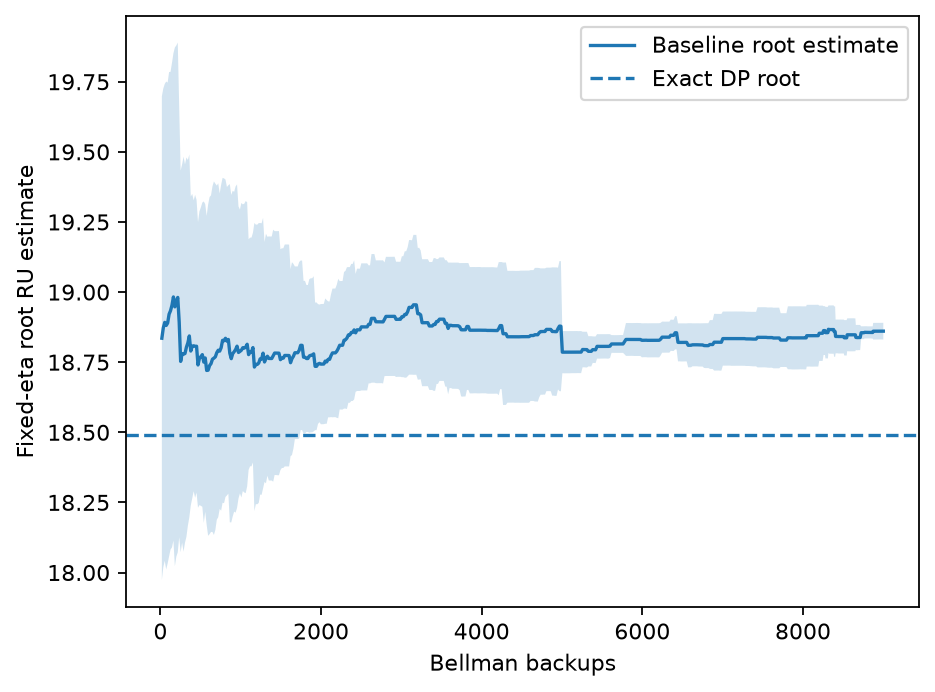
\includegraphics[width=0.78\textwidth]
	{figures/00_validation/root_convergence.png}
	\caption{Root RU estimates with training-seed standard deviations.}
	\label{fig:val-root}
\end{figure}

We evaluate policy quality on 2,000 shared disturbance trajectories. Table~\ref{tab:val} reports paired differences averaged over three training seeds. The root RU error is the mean absolute prediction error. The RU and AVaR gaps compare evaluated policies using the fixed threshold and empirical AVaR, respectively. Positive gaps favor exact DP.

\begin{table}[H]
	\centering
	\caption{Baseline errors relative to exact DP.}
	\label{tab:val}
	\begin{tabular}{rrrrr}
		\hline
		Backups &
		Root RU error &
		RU gap &
		AVaR gap &
		Mean-cost gap \\
		\hline
		900   & 0.4934 & 0.0065 & 0.0055 & 0.0114 \\
		1,800 & 0.2965 & 0.0191 & 0.0166 & 0.0074 \\
		2,700 & 0.4030 & 0.0145 & 0.0111 & 0.0035 \\
		3,600 & 0.3903 & 0.0201 & 0.0166 & 0.0111 \\
		5,400 & 0.3035 & 0.0065 & 0.0055 & 0.0114 \\
		7,200 & 0.3429 & 0.0065 & 0.0055 & 0.0114 \\
		8,998 & 0.3696 & 0.0065 & 0.0055 & 0.0114 \\
		\hline
	\end{tabular}
\end{table}

The backup counts are averaged across seeds. Policy gaps remain small at all budgets, with no clear improvement as the budget increases. In contrast, root-value errors are noticeably larger.

Paired evaluation is important: the exact policy has an empirical AVaR of $19.6384$ on the shared sample, compared with $18.4900$ under full path enumeration. Thus, direct comparison with the enumerated value would mix policy and Monte Carlo errors.

Figure~\ref{fig:val-policy} shows the paired policy gaps. All 95\% Monte Carlo intervals for RU differences include zero. However, baseline evaluation may depend on the order in which states are visited because of random initialization and caching. Therefore, these results should be interpreted with caution and do not establish equal policy performance.

\begin{figure}[H]
	\centering
	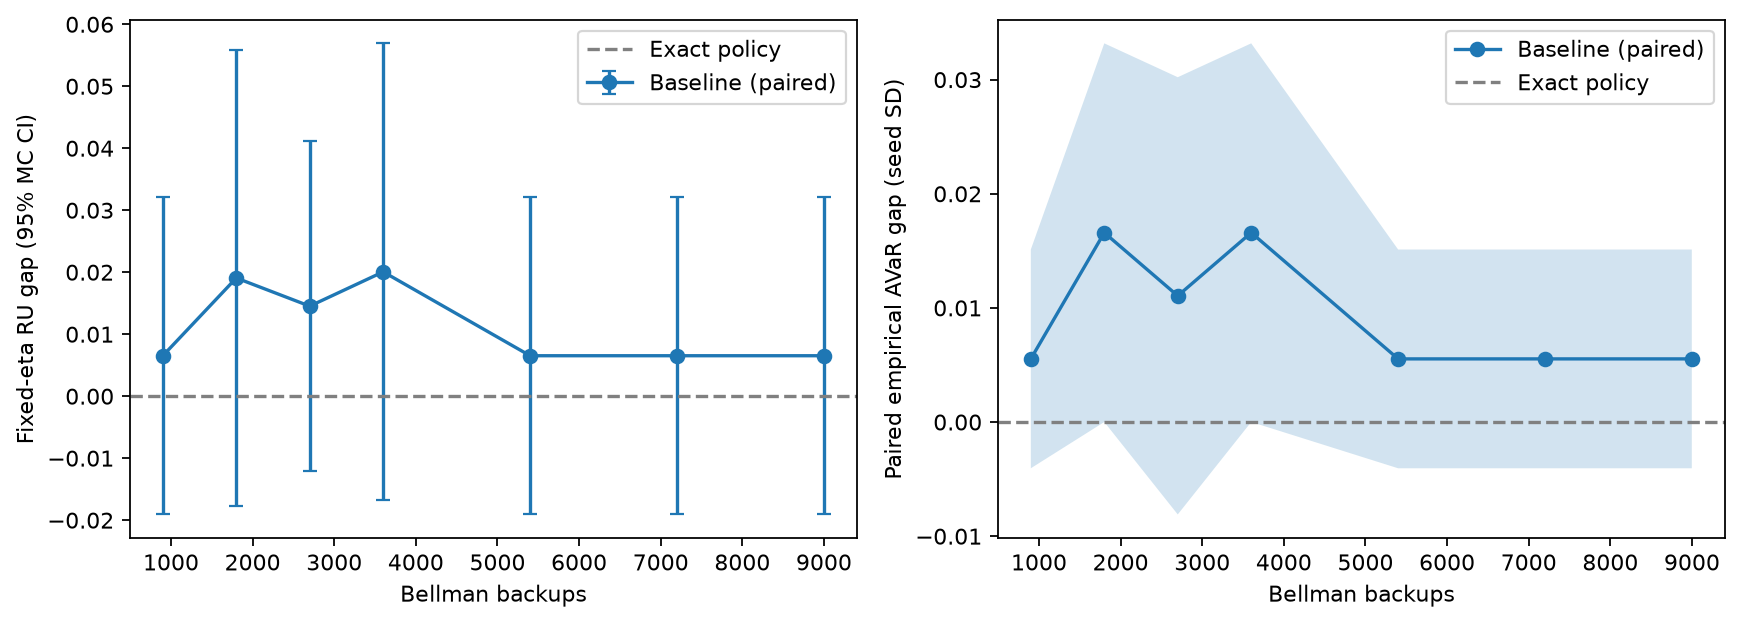
\includegraphics[width=\textwidth]
	{figures/00_validation/policy_performance.png}
	\caption{Paired policy gaps. Left: nominal 95\% Monte Carlo
		intervals. Right: training-seed standard deviations.}
	\label{fig:val-policy}
\end{figure}

The baseline also agrees with the exact policy at all 101 sampled test entries, for every seed and budget.

Overall, baseline ADP achieves policy performance close to exact DP despite noticeable root-value errors.

\subsection{Fixed-threshold probabilistic ADP}
\label{res:fixed}

We compare six probabilistic ADP sampling rules at $\eta=13.75$ for $T=3$ and $\eta=27.8325$ for $T=7$, evaluating policy quality across Bellman-backup budgets.

\paragraph{Empirical AVaR and RU objective.}

Figure~\ref{fig:fixed-risk} shows empirical AVaR and evaluated fixed-threshold RU objectives, both calculated from policy rollouts. For $T=3$, decision-aware sampling gives lower AVaR than random and uncertainty sampling at every budget. At 3,597 backups, the mean values are $19.7929$, $20.4940$, and $20.7308$, respectively. Decision-aware performance is already good at the smallest budget and changes little afterward.

For $T=7$, decision-aware AVaR decreases from $42.4413$ at 885 backups to $36.7091$ at 8,985 backups. At 3,585 backups, it achieves $36.8594$, compared with $40.4588$ for random and $52.4161$ for uncertainty sampling.

\begin{figure}[H]
	\centering
	\begin{subfigure}[b]{0.48\textwidth}
		\centering
		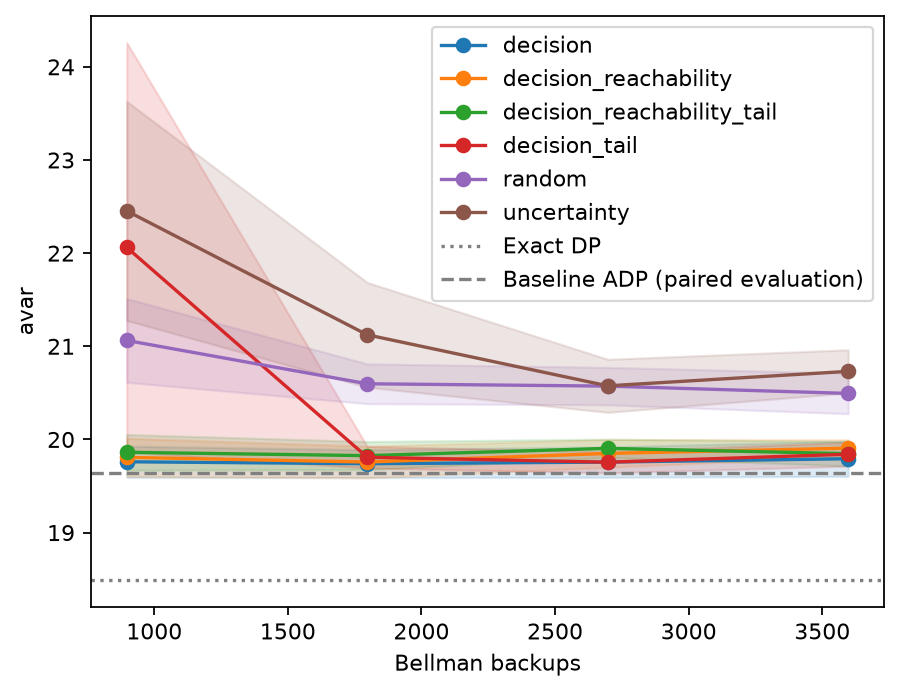
\includegraphics[width=\linewidth]{figures/01_fixed_eta/t3/avar_vs_backups.png}
		\caption{Empirical AVaR, $T=3$.}
		\label{fig:fixed-risk-avar-t3}
	\end{subfigure}
	\hfill
	\begin{subfigure}[b]{0.48\textwidth}
		\centering
		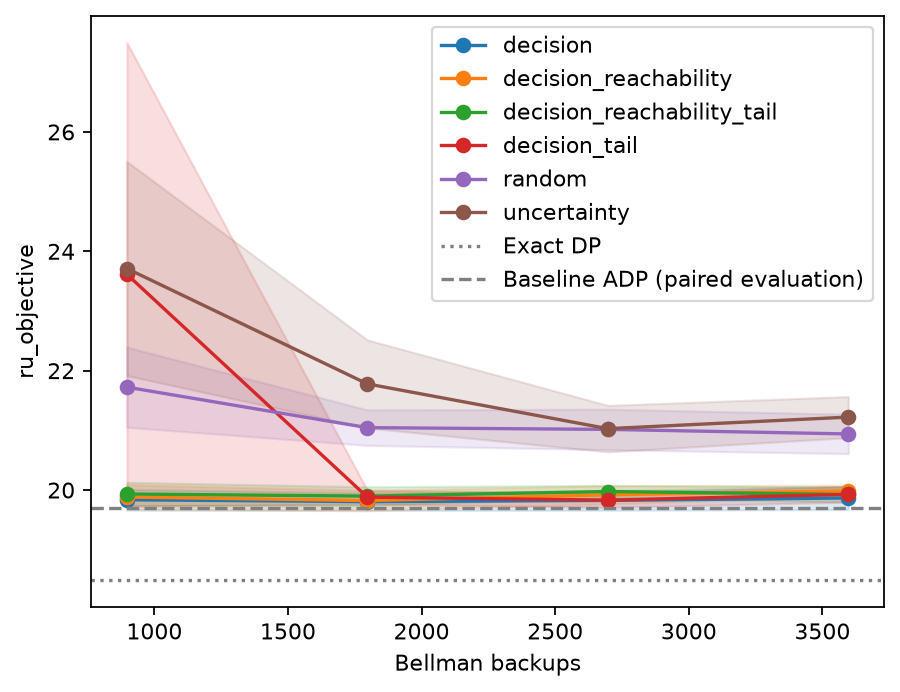
\includegraphics[width=\linewidth]{figures/01_fixed_eta/t3/ru_objective_vs_backups.png}
		\caption{Evaluated RU, $T=3$.}
		\label{fig:fixed-risk-ru-t3}
	\end{subfigure}
	
	\medskip
	
	\begin{subfigure}[b]{0.48\textwidth}
		\centering
		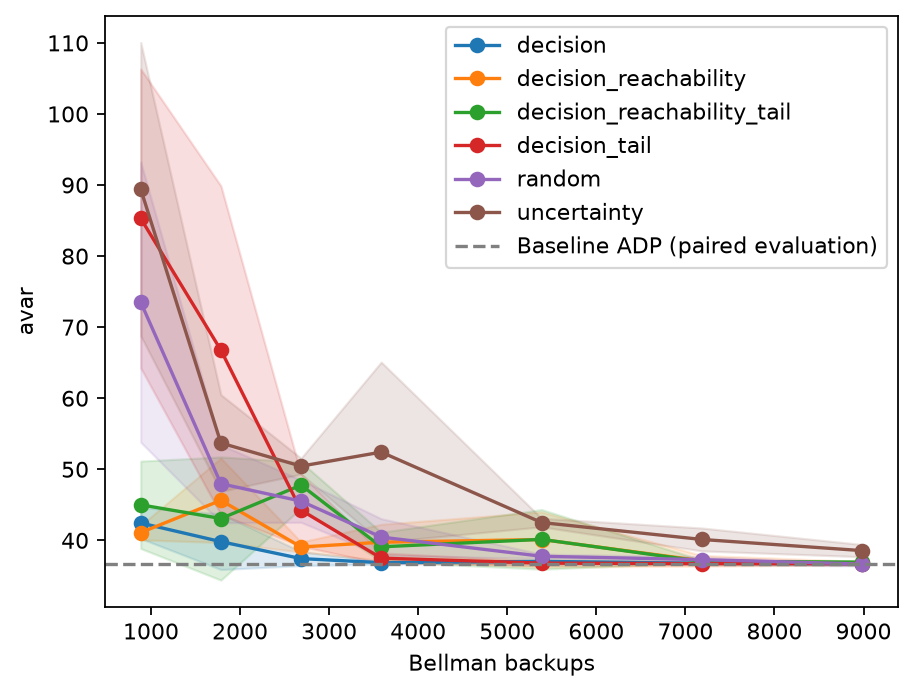
\includegraphics[width=\linewidth]{figures/01_fixed_eta/t7/avar_vs_backups.png}
		\caption{Empirical AVaR, $T=7$.}
		\label{fig:fixed-risk-avar-t7}
	\end{subfigure}
	\hfill
	\begin{subfigure}[b]{0.48\textwidth}
		\centering
		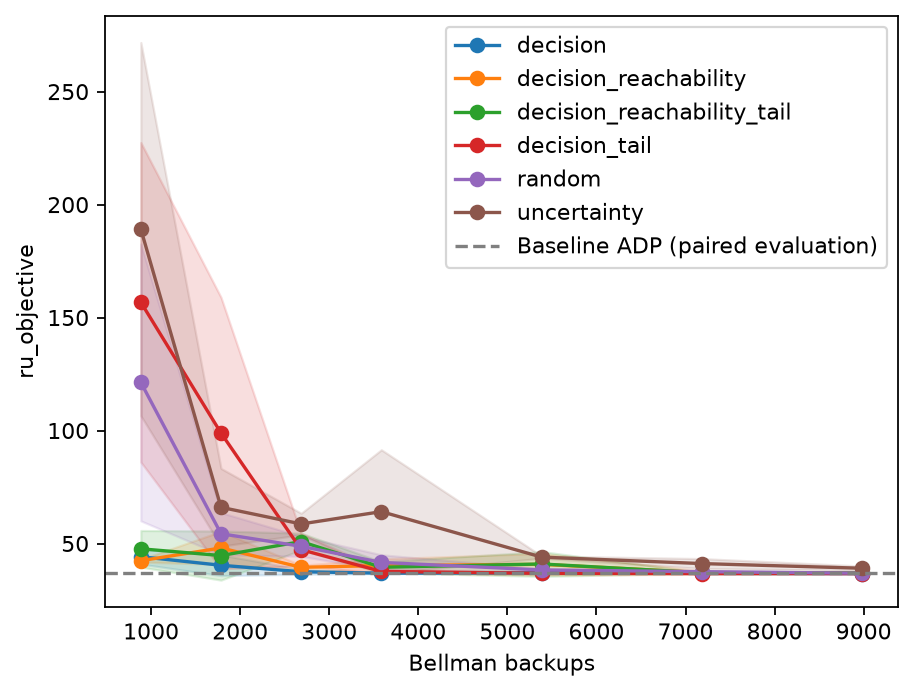
\includegraphics[width=\linewidth]{figures/01_fixed_eta/t7/ru_objective_vs_backups.png}
		\caption{Evaluated RU, $T=7$.}
		\label{fig:fixed-risk-ru-t7}
	\end{subfigure}
	
	\caption{Empirical AVaR and evaluated RU objective against Bellman backups. Shading shows training-seed standard deviations.}
	\label{fig:fixed-risk}
\end{figure}

\paragraph{Comparison with exact DP.}

For $T=3$, the exact policy has AVaR $18.4900$ under full enumeration, but $19.6384$ on the shared 2,000-trajectory evaluation sample. Thus, comparing GP results directly with the enumerated reference includes significant Monte Carlo error.

Figure~\ref{fig:fixed-exact} shows paired RU gaps against exact DP. At 3,597 backups, decision-aware sampling has a mean gap of $0.1704$, with approximate 95\% Monte Carlo interval $[-0.0137,0.3545]$. Random and uncertainty sampling give larger gaps of $1.2430$ and $1.5251$, with intervals above zero. All decision-aware intervals include zero, but this does not establish equality with the exact policy. The intervals measure Monte Carlo uncertainty after averaging across training seeds.

\begin{figure}[H]
	\centering
	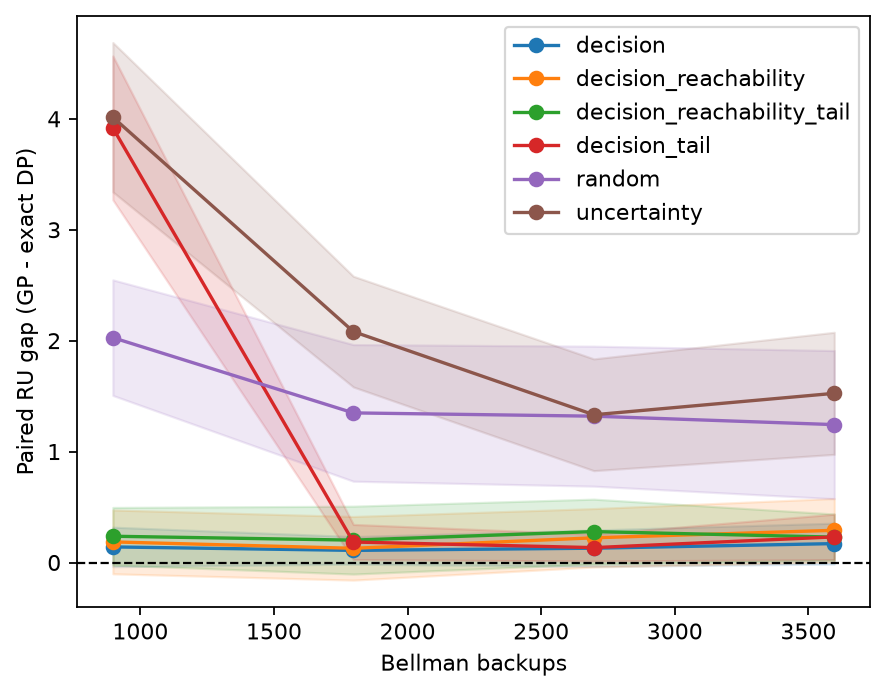
\includegraphics[width=0.78\textwidth]
	{figures/01_fixed_eta/t3/paired_exact_ru_vs_backups.png}
	\caption{Paired RU gaps against exact DP at $T=3$,
		with approximate 95\% Monte Carlo intervals.}
	\label{fig:fixed-exact}
\end{figure}

\paragraph{Comparison with baseline ADP.}

Table~\ref{tab:fixed-paired} reports paired differences against saved baseline policies at the largest budgets. Negative gaps favor probabilistic ADP. The reference uses three baseline policies for $T=3$ and one for $T=7$.

\begin{table}[H]
	\centering
	\caption{Paired gaps relative to baseline ADP.}
	\label{tab:fixed-paired}
	\begin{tabular}{lrrrr}
		\hline
		& \multicolumn{2}{c}{$T=3$: 3,597 backups}
		& \multicolumn{2}{c}{$T=7$: 8,985 backups} \\
		Method & AVaR gap & RU gap & AVaR gap & RU gap \\
		\hline
		Random
		& 0.8500 & 1.2365 & -0.0636 & 0.1058 \\
		Uncertainty
		& 1.0869 & 1.5186 & 1.8196 & 2.3121 \\
		Decision
		& 0.1489 & 0.1639 & -0.0255 & -0.0203 \\
		Decision + reachability
		& 0.2625 & 0.2837 & 0.0558 & 0.0553 \\
		Decision + tail
		& 0.1972 & 0.2242 & -0.0086 & -0.0082 \\
		Decision + reachability + tail
		& 0.2034 & 0.2223 & 0.2043 & 0.2037 \\
		\hline
	\end{tabular}
\end{table}

For $T=7$, decision-aware sampling approaches baseline performance by 3,585 backups. At the largest budget, its gaps are slightly negative but small relative to training-seed variation (standard deviations $0.2956$ for AVaR and $0.3051$ for RU). Random sampling gives a slightly lower empirical AVaR at this budget, but a higher RU objective and mean cost.

Figure~\ref{fig:fixed-paired} shows these comparisons across budgets. They remain descriptive because baseline evaluation can depend on randomized initialization and caching. The $T=7$ baseline is not an exact reference.

\begin{figure}[H]
	\centering
	\begin{subfigure}[b]{0.48\textwidth}
		\centering
		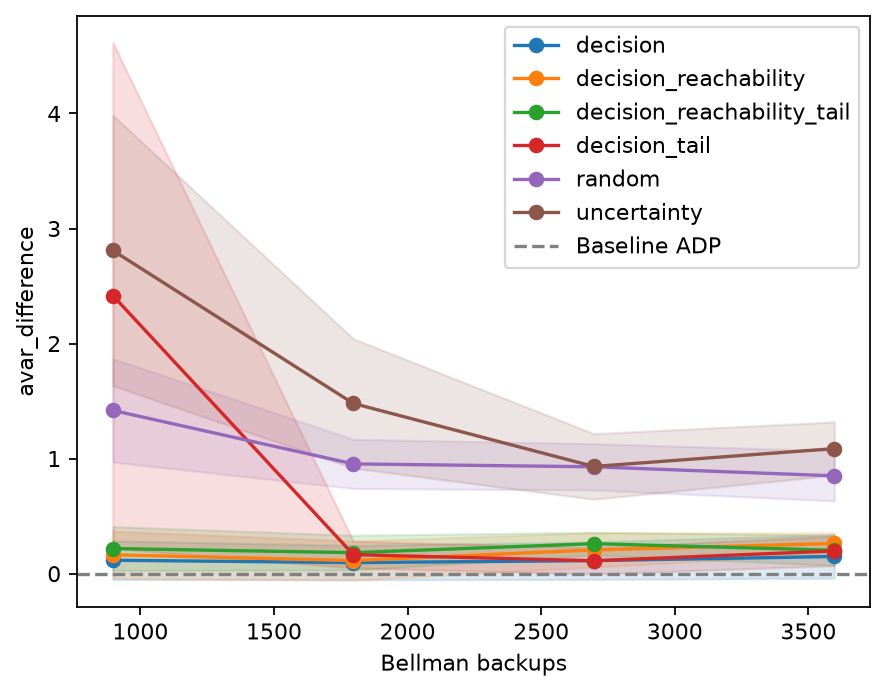
\includegraphics[width=\linewidth]{figures/01_fixed_eta/t3/paired_avar_difference_vs_backups.png}
		\caption{AVaR gaps, $T=3$.}
		\label{fig:fixed-paired-avar-t3}
	\end{subfigure}
	\hfill
	\begin{subfigure}[b]{0.48\textwidth}
		\centering
		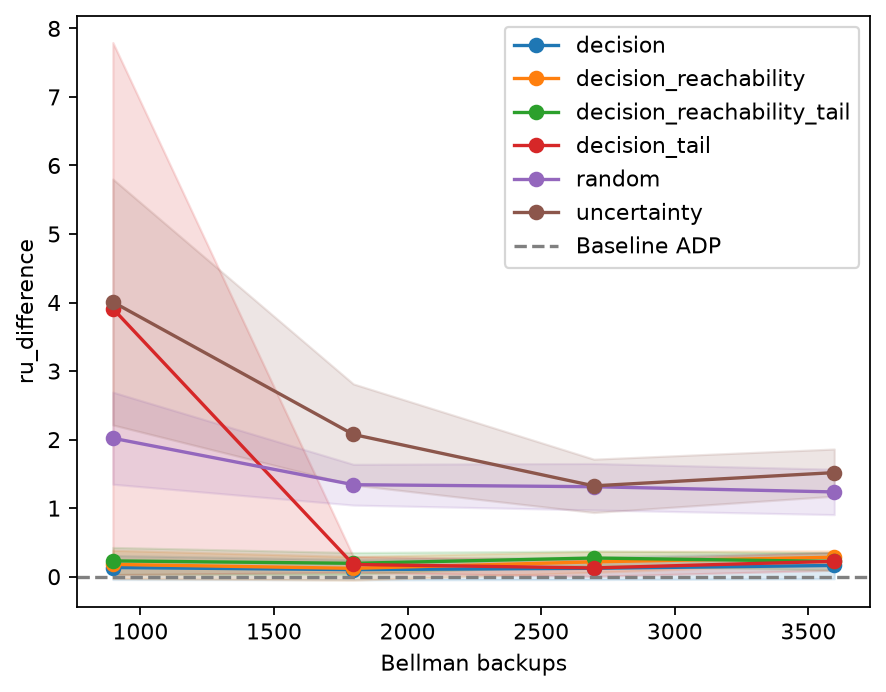
\includegraphics[width=\linewidth]{figures/01_fixed_eta/t3/paired_ru_difference_vs_backups.png}
		\caption{RU gaps, $T=3$.}
		\label{fig:fixed-paired-ru-t3}
	\end{subfigure}
	
	\medskip
	
	\begin{subfigure}[b]{0.48\textwidth}
		\centering
		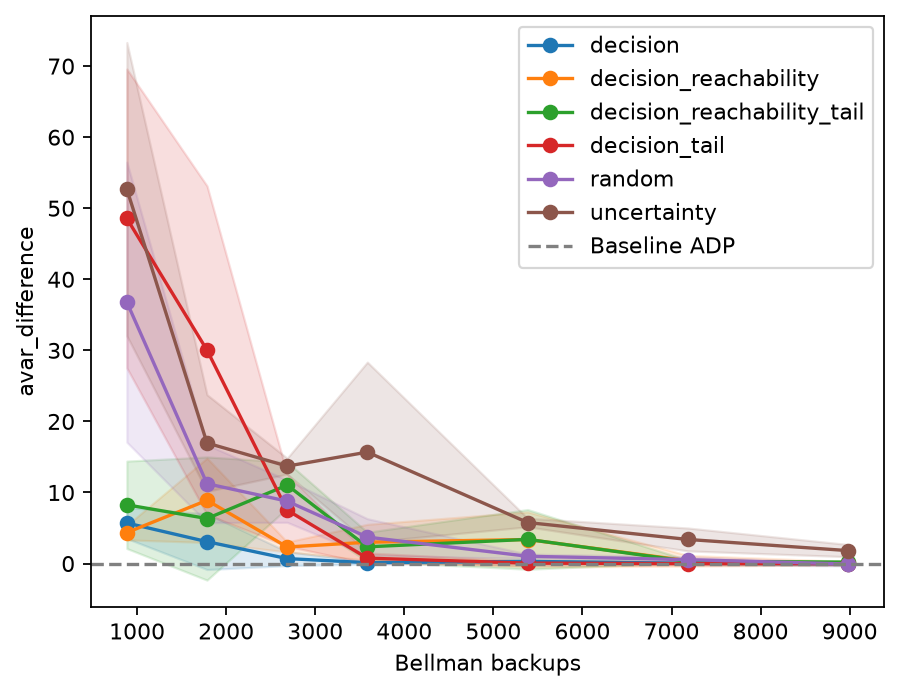
\includegraphics[width=\linewidth]{figures/01_fixed_eta/t7/paired_avar_difference_vs_backups.png}
		\caption{AVaR gaps, $T=7$.}
		\label{fig:fixed-paired-avar-t7}
	\end{subfigure}
	\hfill
	\begin{subfigure}[b]{0.48\textwidth}
		\centering
		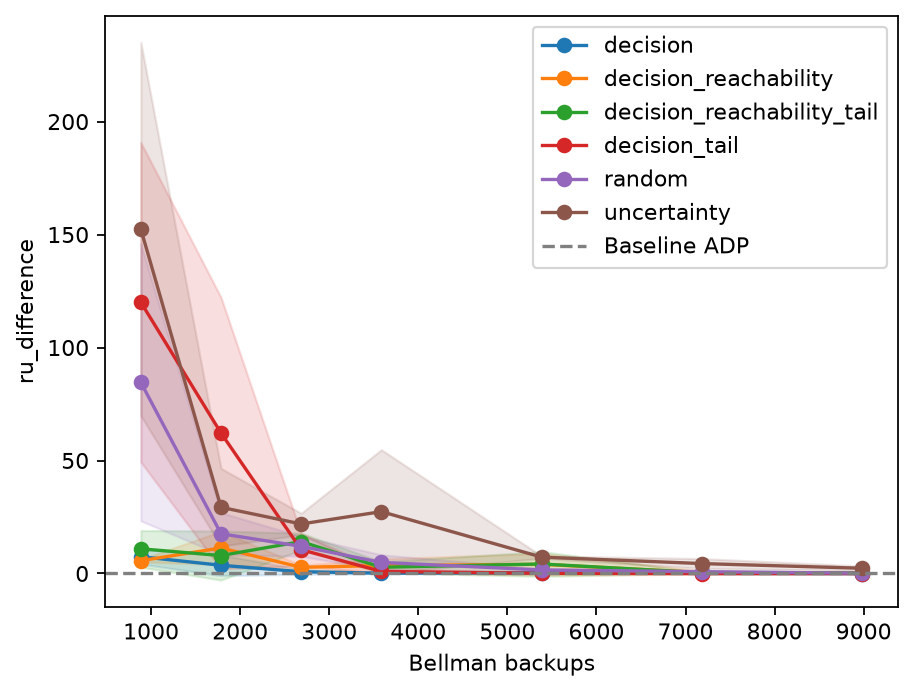
\includegraphics[width=\linewidth]{figures/01_fixed_eta/t7/paired_ru_difference_vs_backups.png}
		\caption{RU gaps, $T=7$.}
		\label{fig:fixed-paired-ru-t7}
	\end{subfigure}
	
	\caption{Paired AVaR and RU gaps to baseline ADP. Shading shows training-seed standard deviations.}
	\label{fig:fixed-paired}
\end{figure}

\paragraph{Acquisition rules and computational cost.}

Adding reachability or tail relevance does not consistently improve decision-aware sampling. Tail weighting is particularly unstable at small budgets, giving mean AVaR $85.2944$ for $T=7$ at 885 backups.

At $T=3$ and 3,597 backups, decision-aware sampling disagrees with the exact policy on only $4.46\%$ of sampled test entries, compared with $38.61\%$ for random and $40.10\%$ for uncertainty sampling.

Predicted objectives also differ from evaluated risk. For decision-aware sampling at $T=7$ and 8,985 backups, predicted and evaluated RU objectives are $38.6927$ and $36.7169$, respectively.

The saved baselines use approximately 18,000 training backups for $T=3$ and 41,766 for $T=7$. Decision-aware GP sampling achieves comparable policy performance with substantially fewer backups and lower recorded training times in these runs. However, this does not establish general speedup factors or the minimum baseline budget needed.

Within probabilistic ADP, active sampling has additional computational costs. At 8,985 backups and $T=7$, decision-aware training takes about 243 seconds, compared with 60 seconds for random sampling. Thus, backup efficiency does not necessarily imply runtime efficiency.

\subsection{Outer-threshold optimization}
\label{res:outer}

We compare random, uncertainty, and decision-aware sampling over $\mathcal{H}=\{0,0.25,\dots,40\}$, using one collection of GP models for all thresholds. The threshold minimizing the predicted RU objective is selected, and its policy is evaluated over shared trajectories.

The outer search requires 483 root backups. At the smallest budget of 897 backups, only 414 remain for GP training.

\paragraph{Selected thresholds.}

Figure~\ref{fig:outer-eta} shows the selected thresholds. At 8,997 backups, decision-aware sampling gives mean $\hat{\eta}=13.525$ for $T=3$, close to the exact grid-optimal value $13.75$. For $T=7$, it gives $\hat{\eta}=27.850$, close to the heuristic pilot value $27.8325$. Neither agreement establishes optimality beyond the available reference.

One random-sampling run at the smallest $T=7$ budget selects the upper boundary $\eta=40$, indicating a possible limitation of the search interval.

\begin{figure}[H]
	\centering
	\begin{subfigure}[b]{0.48\textwidth}
		\centering
		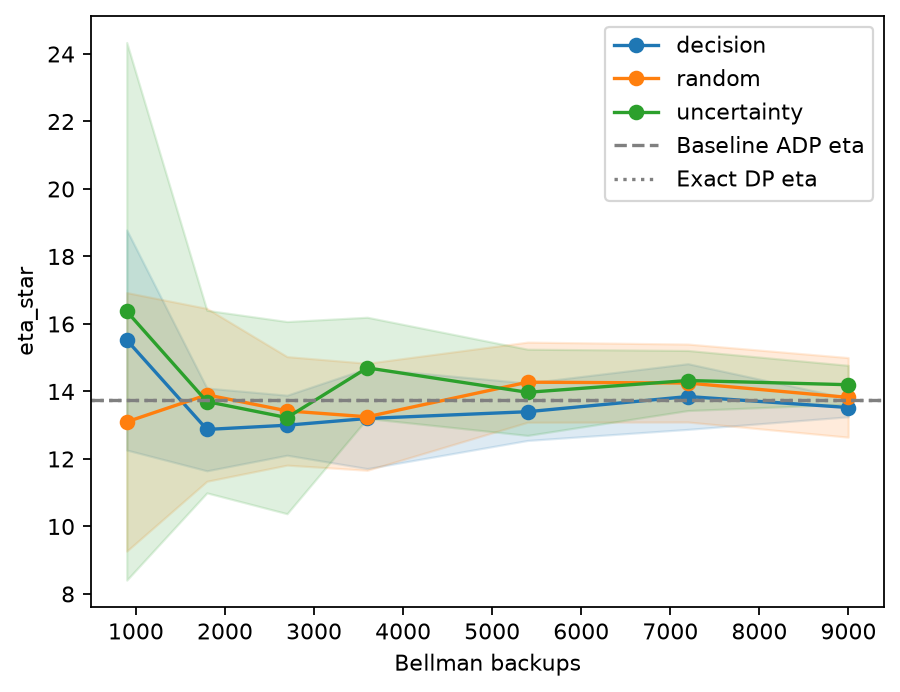
\includegraphics[width=\linewidth]{figures/02_outer_eta/t3/eta_vs_backups.png}
		\caption{Selected thresholds, $T=3$.}
		\label{fig:outer-eta-t3}
	\end{subfigure}
	\hfill
	\begin{subfigure}[b]{0.48\textwidth}
		\centering
		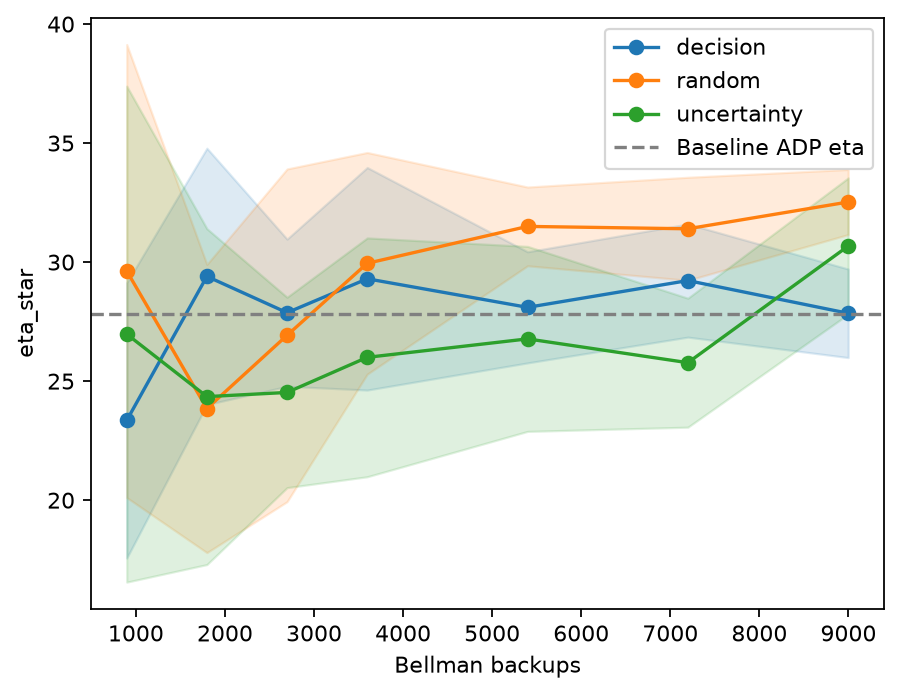
\includegraphics[width=\linewidth]{figures/02_outer_eta/t7/eta_vs_backups.png}
		\caption{Selected thresholds, $T=7$.}
		\label{fig:outer-eta-t7}
	\end{subfigure}
	
	\caption{Selected thresholds against Bellman backups. Shading shows training-seed standard deviations.}
	\label{fig:outer-eta}
\end{figure}

\paragraph{Predicted and evaluated objectives.}

Figure~\ref{fig:outer-ru} compares predicted minimum RU objectives with those evaluated from policy rollouts. After GP training, predictions require only root Bellman evaluations, without Monte Carlo policy rollouts. Their cost is independent of the evaluation sample size.

However, predictions are not always accurate. For $T=3$ at 897 backups, random sampling predicts $17.8852$, below the exact grid minimum $18.4911$, while its evaluated RU is $28.3359$. At the largest budget, decision-aware sampling gives predicted and evaluated RU values of $18.8761$ and $20.1483$ for $T=3$, and $38.3366$ and $36.7794$ for $T=7$. These differences reflect both approximation and Monte Carlo evaluation errors, which are not separated in this experiment.

\begin{figure}[H]
	\centering
	\begin{subfigure}[b]{\textwidth}
		\centering
		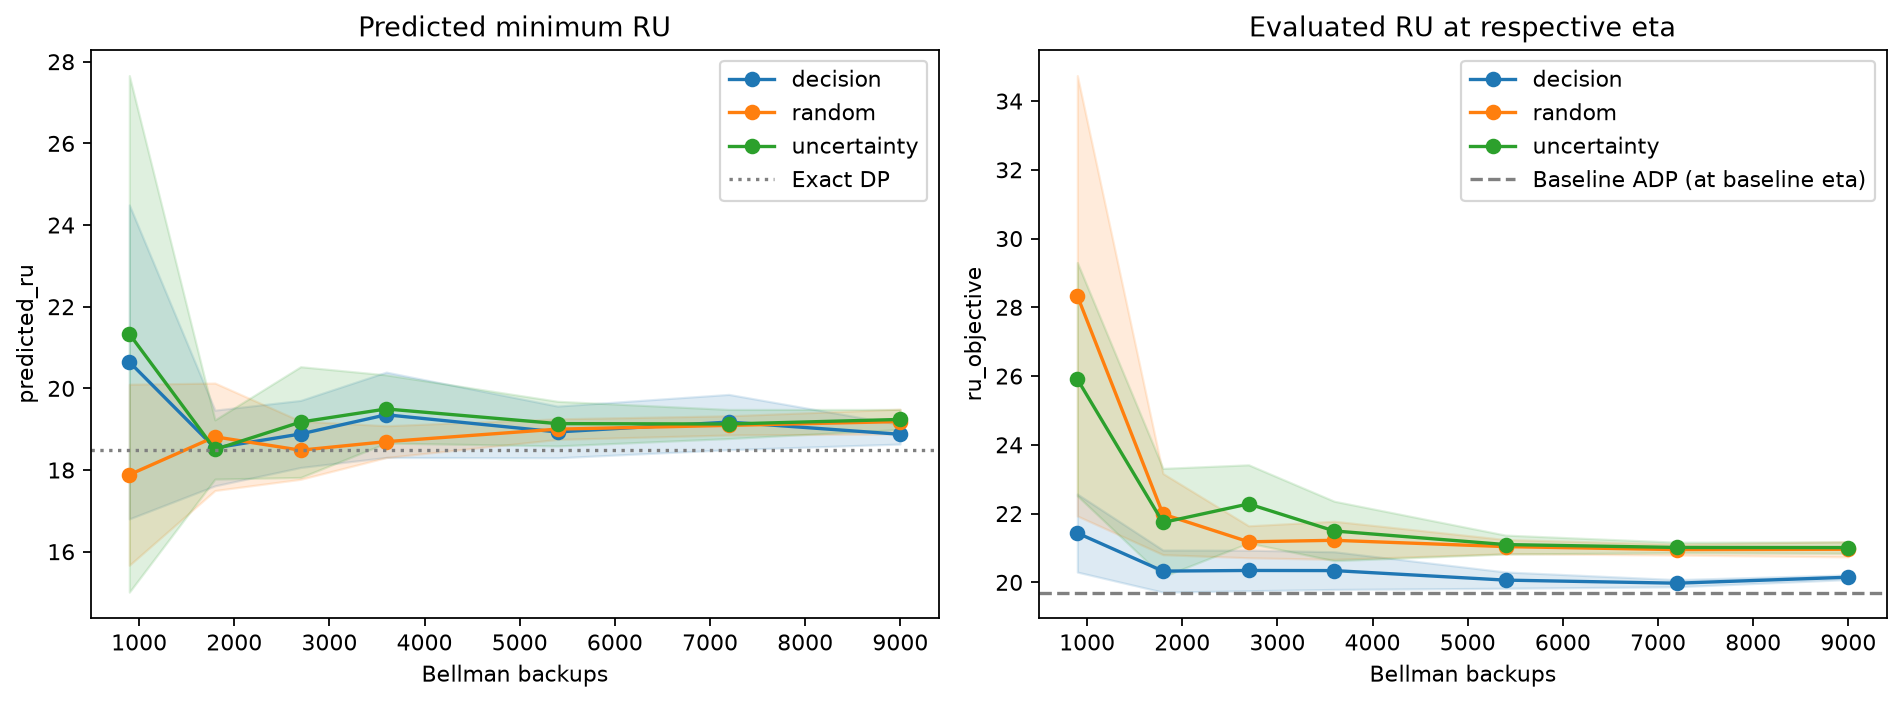
\includegraphics[width=\linewidth]{figures/02_outer_eta/t3/ru_vs_backups.png}
		\caption{Predicted minimum and evaluated RU, $T=3$.}
		\label{fig:outer-ru-t3}
	\end{subfigure}
	
	\medskip
	
	\begin{subfigure}[b]{\textwidth}
		\centering
		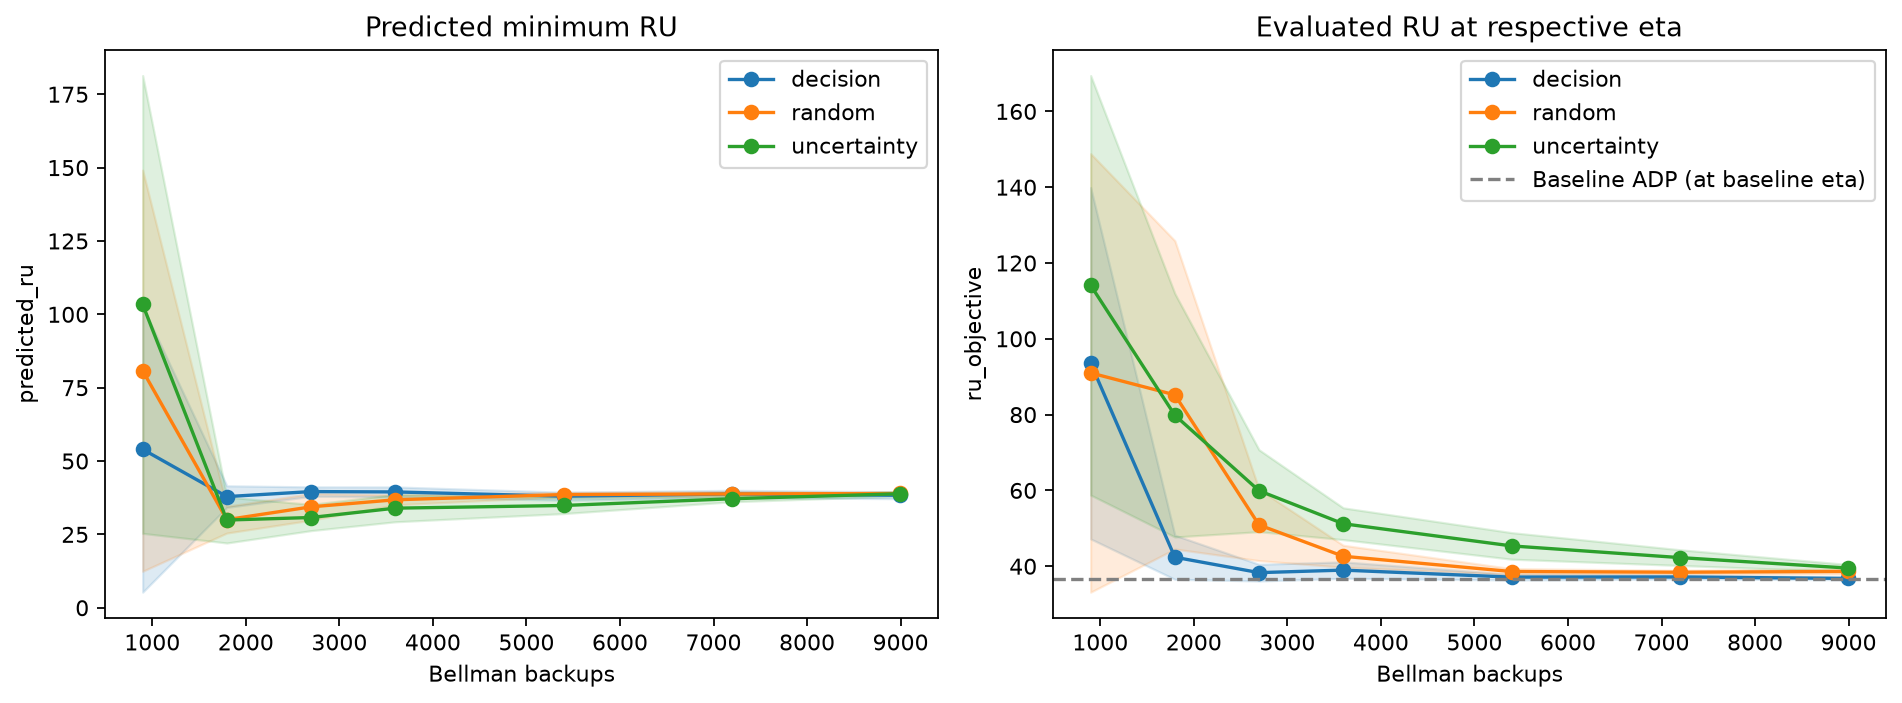
\includegraphics[width=\linewidth]{figures/02_outer_eta/t7/ru_vs_backups.png}
		\caption{Predicted minimum and evaluated RU, $T=7$.}
		\label{fig:outer-ru-t7}
	\end{subfigure}
	
	\caption{Predicted minimum RU (left) and evaluated RU (right) against Bellman backups. Shading shows training-seed standard deviations.}
	\label{fig:outer-ru}
\end{figure}

\paragraph{Evaluated policy performance.}

Table~\ref{tab:outer} reports the results at the largest budget. Decision-aware sampling achieves the lowest mean empirical AVaR and mean cost for both horizons. For $T=7$, its AVaR decreases from $57.2183$ at 897 backups to $36.5893$ at 8,997 backups. The improvement is less consistent for $T=3$.

\begin{table}[H]
	\centering
	\caption{Outer-threshold results at 8,997 backups.
		Means across ten training seeds.}
	\label{tab:outer}
	\begin{tabular}{llrrrr}
		\hline
		$T$ & Method & $\hat{\eta}$ & AVaR & Evaluated RU
		& Mean cost \\
		\hline
		\multirow{3}{*}{3} & Random      & 13.825 & 20.4978 & 20.9621 & 7.4354 \\
		 & Uncertainty & 14.200 & 20.6727 & 21.0112 & 7.5685 \\
		 & Decision    & 13.525 & 19.9907 & 20.1483 & 6.6625 \\
		\hline
		\multirow{3}{*}{7} & Random      & 32.525 & 38.1217 & 38.6228 & 16.1180 \\
		 & Uncertainty & 30.675 & 39.1253 & 39.5088 & 16.7823 \\
		 & Decision    & 27.850 & 36.5893 & 36.7794 & 14.7408 \\
		\hline
	\end{tabular}
\end{table}

\paragraph{Paired evaluation.}

Figure~\ref{fig:outer-paired} compares empirical AVaR against one saved fixed-threshold baseline policy per horizon, using shared disturbance trajectories.

At the largest budget, decision-aware sampling gives mean paired AVaR gaps of $0.3523$ for $T=3$ and $-0.1454$ for $T=7$. The latter has training-seed standard deviation $0.3136$, so it does not establish superiority over the baseline. Random and uncertainty sampling give larger gaps of $1.3871$ and $2.3906$ for $T=7$.

\begin{figure}[H]
	\centering
	\begin{subfigure}[b]{0.48\textwidth}
		\centering
		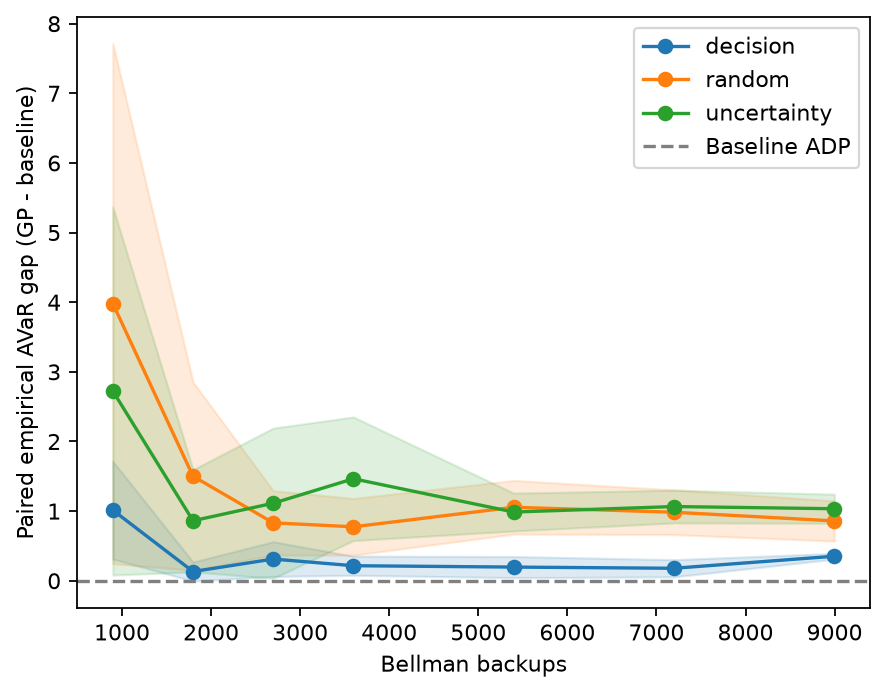
\includegraphics[width=\linewidth]{figures/02_outer_eta/t3/paired_avar_vs_backups.png}
		\caption{Paired AVaR gaps, $T=3$.}
		\label{fig:outer-paired-t3}
	\end{subfigure}
	\hfill
	\begin{subfigure}[b]{0.48\textwidth}
		\centering
		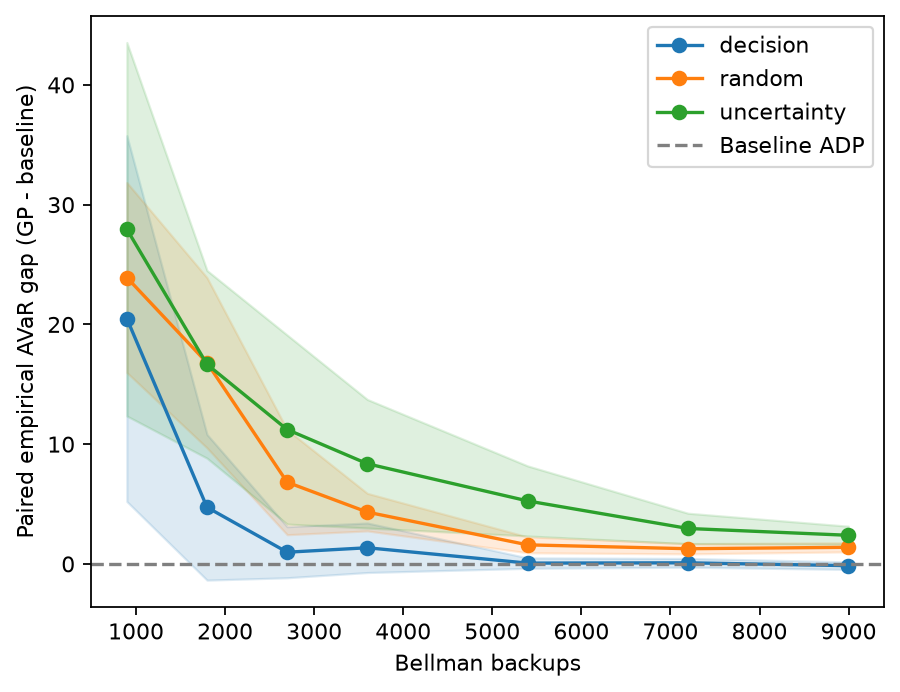
\includegraphics[width=\linewidth]{figures/02_outer_eta/t7/paired_avar_vs_backups.png}
		\caption{Paired AVaR gaps, $T=7$.}
		\label{fig:outer-paired-t7}
	\end{subfigure}
	
	\caption{Paired empirical AVaR gaps to baseline ADP against Bellman backups. Shading shows training-seed standard deviations.}
	\label{fig:outer-paired}
\end{figure}

We also compare RU gaps using the baseline threshold and each policy's own threshold, without changing the policies. For decision-aware sampling at $T=7$ and 8,997 backups, the gaps are $-0.1437$ and $0.0421$, with nominal 95\% Monte Carlo intervals $[-0.8676,0.5803]$ and $[-0.6857,0.7700]$, respectively. Both differences are small relative to their uncertainty, but baseline evaluation may depend on evaluation order. These results also show that the selected threshold does not always minimize the empirical RU objective.

\paragraph{Interpretation and computational cost.}

Decision-aware sampling gives better threshold and policy estimates than the other sampling methods in these experiments. However, we cannot conclude that outer optimization is better than fixed-threshold training, since the experiments use different candidate domains, budgets, and numbers of seeds.

Decision-aware sampling is also slower than random sampling. At the largest budget, mean training times are about 2,219 versus 98 seconds for $T=3$, and 412 versus 100 seconds for $T=7$. The higher runtime for $T=3$ may be explained by the larger number of training points per GP, since the backup budget is distributed across fewer stages. As GP fitting has roughly cubic complexity, training can be slower for shorter horizons despite having fewer stages.


\subsection{Candidate-pool ablation}
\label{res:pool}

We compare random and decision-aware sampling with 1,000 to 5,000 candidates per stage. Smaller pools are subsets of the same 5,000-point pool, with other training settings fixed. We use three training seeds and 20,000 shared evaluation trajectories. Due to different evaluation sample sizes, raw AVaR estimates are not directly compared with earlier experiments.

\paragraph{Effect on decision-aware sampling.}

Figure~\ref{fig:pool-decision} shows empirical AVaR across budgets. For $T=3$, larger pools generally improve performance. At 3,597 backups, increasing the pool from 1,000 to 5,000 candidates reduces mean AVaR from $19.4200$ to $18.8939$ and sampled policy disagreement from $32.01\%$ to $4.62\%$.

For $T=7$, the differences between pool sizes become small as the budget increases. At 8,985 backups, all methods give similar AVaR values, with no clear advantage from larger candidate pools. This suggests that pool size has little effect on policy performance at larger budgets.

\begin{figure}[H]
	\centering
	\begin{subfigure}[b]{0.48\textwidth}
		\centering
		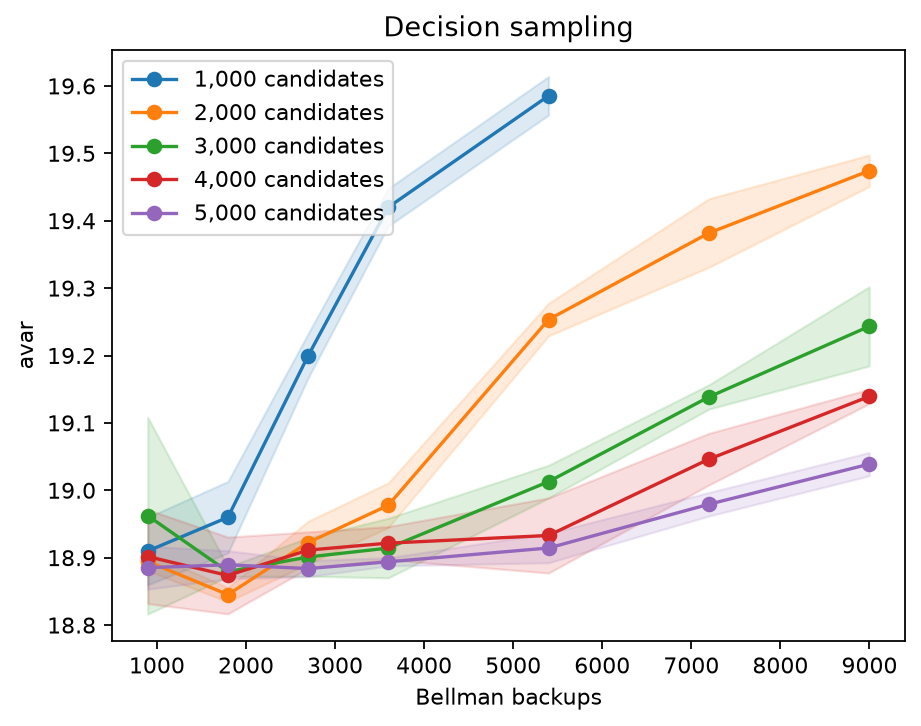
\includegraphics[width=\linewidth]{figures/03_candidate_pool/t3/avar_vs_backups_decision.png}
		\caption{Decision-aware AVaR, $T=3$.}
		\label{fig:pool-decision-t3}
	\end{subfigure}
	\hfill
	\begin{subfigure}[b]{0.48\textwidth}
		\centering
		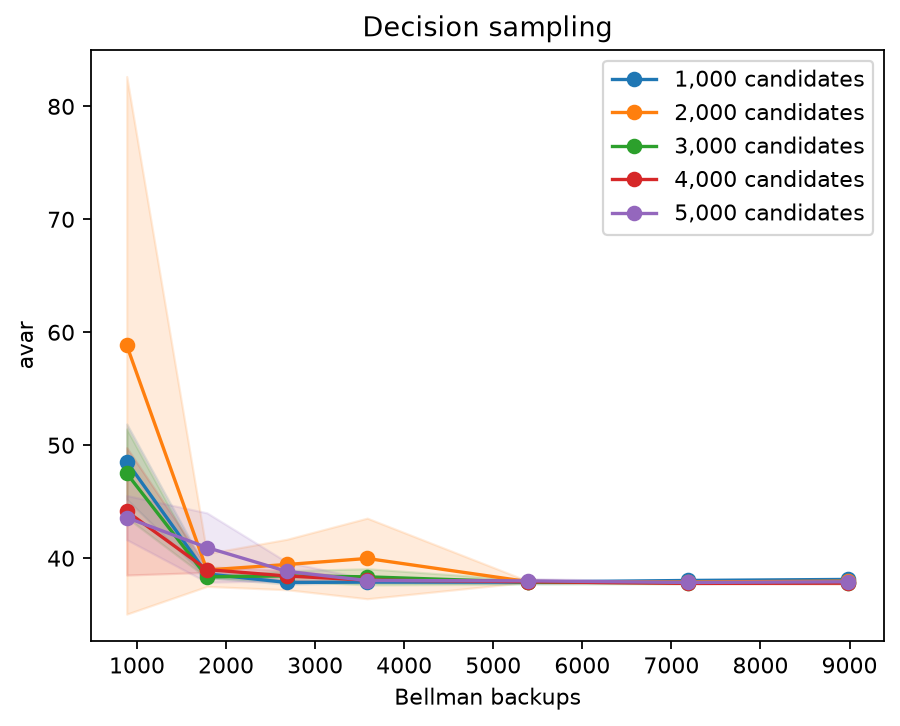
\includegraphics[width=\linewidth]{figures/03_candidate_pool/t7/avar_vs_backups_decision.png}
		\caption{Decision-aware AVaR, $T=7$.}
		\label{fig:pool-decision-t7}
	\end{subfigure}
	
	\caption{Decision-aware AVaR for different pool sizes. Shading shows training-seed standard deviations.}
	\label{fig:pool-decision}
\end{figure}

Table~\ref{tab:pool} summarizes the results at the nominal budget of 3,600 backups.

\begin{table}[H]
	\centering
	\caption{Decision-aware sampling at 3,600 nominal backups.}
	\label{tab:pool}
	\begin{tabular}{rrrr}
		\hline
		Candidates per stage &
		$T=3$ AVaR &
		$T=3$ disagreement (\%) &
		$T=7$ AVaR \\
		\hline
		1,000 & 19.4200 & 32.01 & 37.8834 \\
		2,000 & 18.9777 & 13.20 & 39.9740 \\
		3,000 & 18.9143 &  8.25 & 38.3482 \\
		4,000 & 18.9216 &  7.59 & 38.0603 \\
		5,000 & 18.8939 &  4.62 & 38.0193 \\
		\hline
	\end{tabular}
\end{table}

\paragraph{Paired comparisons between pool sizes.}

Figure~\ref{fig:pool-paired} shows paired empirical AVaR differences relative to the 5,000-point pool, using the same seeds, budgets, and disturbance paths. Positive differences favor the larger pool.

For decision-aware sampling at $T=3$, smaller pools become less effective at larger budgets. At 3,597 backups, the 1,000-point pool has a mean AVaR gap of $0.5261$, with training-seed standard deviation $0.0239$. Random sampling shows no similarly clear ordering, since it does not rank candidates by acquisition scores.

For $T=7$, differences between pools become small at larger budgets. With only three training seeds, the experiment does not establish a reliable ranking of pool sizes.

\begin{figure}[H]
	\centering
	\begin{subfigure}[b]{\textwidth}
		\centering
		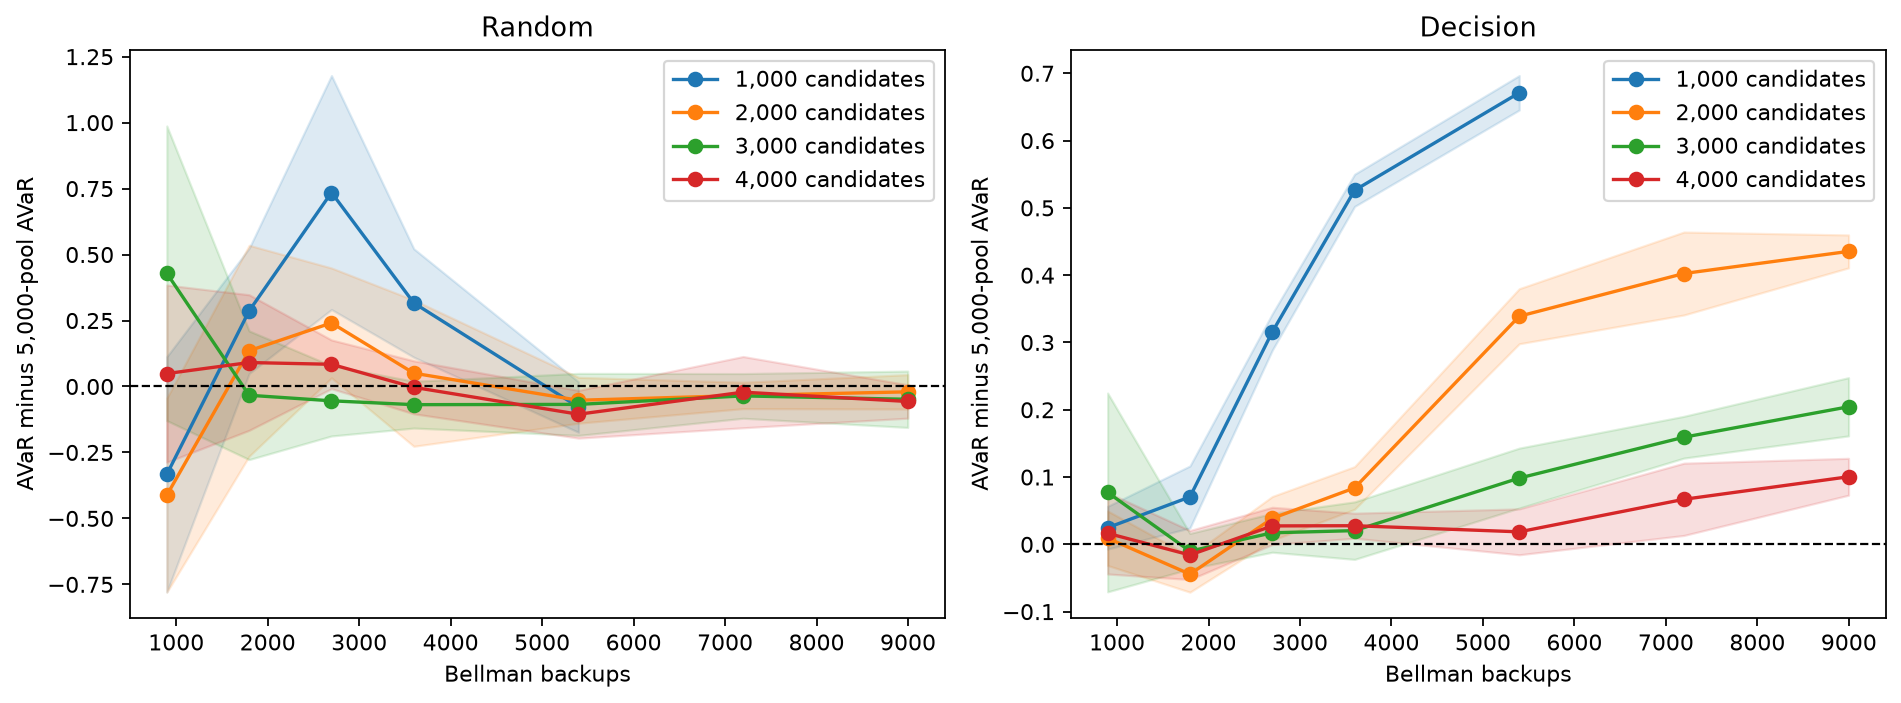
\includegraphics[width=\linewidth]{figures/03_candidate_pool/t3/avar_difference.png}
		\caption{Paired AVaR gaps, $T=3$.}
		\label{fig:pool-paired-t3}
	\end{subfigure}
	
	\medskip
	
	\begin{subfigure}[b]{\textwidth}
		\centering
		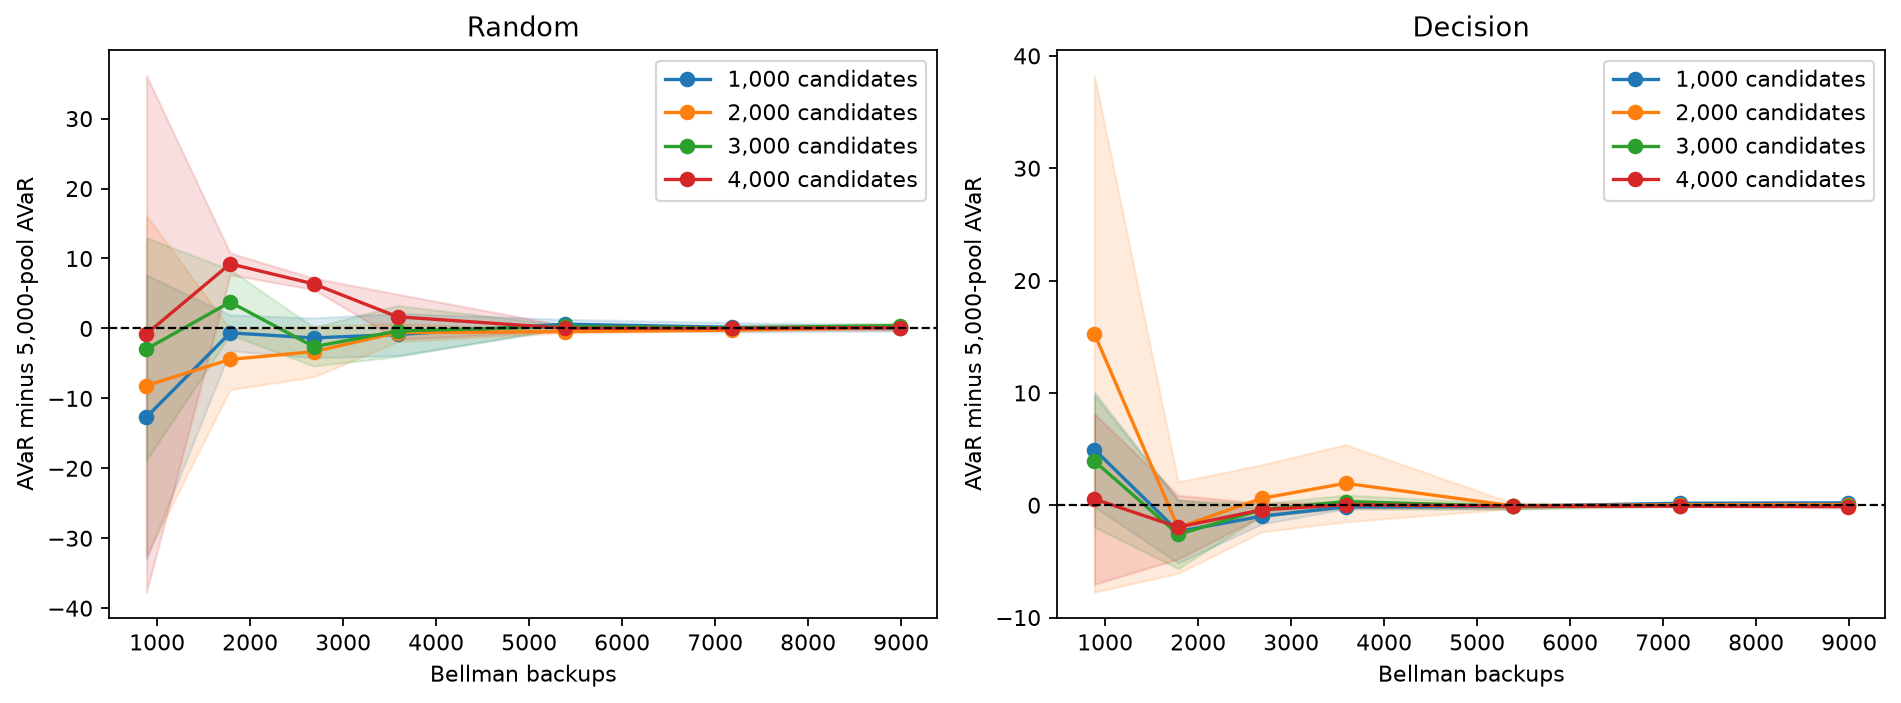
\includegraphics[width=\linewidth]{figures/03_candidate_pool/t7/avar_difference.png}
		\caption{Paired AVaR gaps, $T=7$.}
		\label{fig:pool-paired-t7}
	\end{subfigure}
	
	\caption{Paired AVaR gaps relative to 5{,}000 candidates. Shading shows training-seed standard deviations.}
	\label{fig:pool-paired}
\end{figure}

\paragraph{Pool utilization and increasing budgets.}

More backups do not always improve the policy. For $T=3$, decision-aware AVaR with 1,000 candidates increases from $18.9099$ at 897 backups to $19.5854$ at 5,397 backups. With 5,000 candidates, the increase is smaller, from $18.8852$ to $18.9144$.

At 5,397 backups, the algorithm uses 899 states per stage, corresponding to $89.9\%$ of the smaller pool but only $17.98\%$ of the larger one. High pool utilization leaves less freedom for acquisition, which may contribute to the deterioration.

However, the experiment does not establish its cause. GP refitting and backward propagation of approximate Bellman targets may also contribute. Even with 5,000 candidates, AVaR rises to $19.0388$ at 8,997 backups. Thus, larger pools reduce but do not eliminate the observed deterioration.

Using fewer backups or larger pools may help, but neither guarantees better performance.

\paragraph{Computational trade-off.}

Larger pools increase acquisition costs. At 3,600 nominal backups, increasing the pool from 1,000 to 5,000 candidates raises mean training time from 192 to 257 seconds for $T=3$, and from 68 to 82 seconds for $T=7$, without changing the number of backups.

Candidate-pool size is therefore an additional computational parameter that should be considered together with the Bellman-backup budget.


\subsection{Discussion}
\label{res:discussion}

The main finding is that decision-aware sampling often achieves better policy performance per Bellman backup than random or uncertainty sampling, especially at moderate budgets. Adding reachability or tail weighting does not consistently improve these results.

\paragraph{Value accuracy and policy quality.}

The baseline ADP achieves policy performance close to exact DP despite noticeable root-value errors. This shows that accurate value estimation and accurate action selection are different objectives. As shown by the action-gap result in Section~\ref{theory:action-gap}, approximation errors may preserve the optimal action when they are sufficiently small relative to the true action gap. The experiments are consistent with this result but do not verify the condition at every state.

Outer-threshold optimization additionally depends on the accuracy of the predicted RU objective. A good fixed-threshold policy or a small predicted objective does not guarantee a good selected threshold. The experiments also do not establish that outer optimization improves on fixed-threshold training, since their configurations and budget allocations differ.

\paragraph{Paired evaluation.}

Paired evaluation reduces Monte Carlo noise when comparing policies. For $T=3$, much of the difference from the exact AVaR comes from the finite evaluation sample. However, pairing does not remove actual policy differences or sampling uncertainty.

All training seeds use the same evaluation trajectories, so averaging over seeds does not remove sampling error. Also, empirical AVaR and fixed-threshold RU may rank policies differently because only AVaR minimizes over the threshold.

\paragraph{Reachability and tail weighting.}

The additional scores use trajectories generated by the fitted risk-neutral policy, which may not represent the states important under the AVaR policy. Multiplying these scores by decision uncertainty may also reduce the priority of useful states. Furthermore, threshold exceedance is only a proxy for the effect of action errors on AVaR.

These are possible explanations for the mixed results. Experiments on tail relevance weighting did not show meaningful improvements either. Thus, better ways of incorporating reachability and tail relevance might be a subject for further research.

\paragraph{Candidate pools and computational cost.}

The candidate-pool experiment shows that more Bellman backups do not always improve policy performance. Smaller pools can restrict acquisition when most candidates are already selected. Larger pools reduce the observed deterioration for $T=3$, but do not guarantee improvement. GP refitting and backward propagation of approximation errors may also contribute, although their effects were not isolated.

Backup efficiency also differs from runtime efficiency. Repeated GP fitting and acquisition calculations can make decision-aware sampling slower than random sampling. However, decision-only acquisition avoids the additional rollouts and nearest-neighbor calculations required for reachability and tail scores. Its accuracy and simpler acquisition procedure make it attractive, although the experiments do not establish a consistent accuracy-runtime advantage over the weighted variants.

\paragraph{Further threshold-search improvements.}

The same trained GP models can evaluate the predicted RU objective at different thresholds. An adaptive search could therefore reduce root evaluations and leave more budget for GP training. However, the optimized RU objective is not necessarily convex or unimodal, so local optimization does not guarantee a global minimum.

\paragraph{Limitations.}

The experiments consider one scalar control problem, two horizons, and one confidence level. Exact DP is available only for $T=3$ under discretized disturbances, and its threshold is grid-optimal. For $T=7$, the fixed threshold is heuristic, and its pilot estimation shares an evaluation seed with later benchmarks.

Baseline evaluation may randomly initialize and cache unseen states. Evaluation-order dependence was confirmed for the saved $T=7$ policy, but its effect on benchmark rankings was not established. Baseline comparisons and their Monte Carlo intervals therefore require caution.

GP uncertainty is model-based and does not guarantee small Bellman approximation errors. The risk-neutral continuation is also approximated, despite the exact mathematical decomposition for $y\geq0$. Finally, some experiments use only three training seeds, and shared evaluation trajectories introduce common Monte Carlo uncertainty.

Thus, the results support decision-aware Bellman allocation within the tested settings, without establishing general superiority or convergence. The main remaining question is how reachability and tail information can improve policy accuracy beyond decision uncertainty alone.

	
	\section{Conclusion}
\label{sec:conclusion}

In this paper, we studied finite-horizon static AVaR control using approximate dynamic programming. We proposed a probabilistic ADP method based on Gaussian processes, which approximates Q-functions in the difficult region of the augmented state space and allocates Bellman backups according to decision uncertainty, reachability, and tail relevance. We also derived approximation and policy-performance error bounds, accounting for the risk-neutral decomposition and outer threshold optimization.

The experiments show that decision-aware sampling often achieves better policy performance per Bellman backup than random or uncertainty sampling, especially at moderate computational budgets. However, adding reachability or tail weighting does not consistently improve performance. We also observed that better value-function estimates do not necessarily produce better policies, and that increasing the number of Bellman backups does not always improve the resulting AVaR.

These findings suggest that allocating computational effort according to uncertainty about the optimal action is a promising approach to risk-averse ADP. Nevertheless, the experiments are limited to one control problem and do not establish general superiority or convergence. Future work may investigate more effective ways to incorporate reachability and tail relevance, as well as extensions to more complex control problems.
	
	\section*{Code availability}

The source code and experimental scripts used in this
study are publicly available at \\ \url{https://github.com/dilzhan/avar-mdp}.
	
	\newpage
	\bibliographystyle{plainnat}
	\bibliography{ref}
	
	\appendix
	
	\section{Baseline ADP}
\label{app:baseline-adp}

\begin{algorithm}[H]
	\caption{Baseline ADP}
	\label{alg:baseline-adp}
	\begin{algorithmic}[1]
		\Require Initial state $x_0$, threshold $\eta$,
		number of episodes $K$, number of initialization rollouts $N$.
		\Ensure Cache $\mathcal{C}$.
		\State Initialize cache $\mathcal{C} \gets \varnothing$
		
		\For{$k = 1, \ldots, K$}
		\State $(x,y) \gets (x_0,-\eta)$
		
		\For{$t = 0, \ldots, T-1$}
		\State $s \gets (t, \operatorname{Round}(x, y))$
		\For{$a \in \mathcal{A}$}
		\State $\displaystyle q(a) \gets
		\sum_{i} w_i
		\Call{Value}{
			t+1,
			f_t(x,a,\xi^{(i)}),
			y+c_t(x,a)
		}$
		\EndFor
		
		\State $\displaystyle a_t \gets
		\arg\min_{a \in \mathcal{A}} q(a)$
		
		\If{$y < 0$}
		\State $\displaystyle \mathcal{C}[s]
		\gets \min_{a \in \mathcal{A}} q(a)$
		\EndIf
		
		\State Sample $\xi_t$ from $\Xi$ with probabilities $w_i$
		\State $y \gets y+c_t(x,a_t)$
		\State $x \gets f_t(x,a_t,\xi_t)$
		\EndFor
		\EndFor
		
		\State \Return $\mathcal{C}$
		
		\Statex
		
		\Function{Value}{$t,x,y$}
		\If{$t=T$}
		\State \Return $(y+c_T(x))_+$
		\EndIf
		
		\If{$y \geq 0$}
		\State \Return $y+\hat V_t^{\text{RN}}(x)$
		\EndIf
		
		\State $s \gets (t,\operatorname{Round}(x,y))$
		
		\If{$s \notin \mathcal{C}$}
		\State $\mathcal{C}[s] \gets
		\Call{Initialize}{t,x,y,N}$
		\EndIf
		
		\State \Return $\mathcal{C}[s]$
		\EndFunction
	\end{algorithmic}
\end{algorithm}

Here, $\Xi = \{\xi^{(i)}\}_{i=0}^{N_{\xi}}$ is the discretized noise range, and $w_i$ are the corresponding normalized probability weights $w_i = \frac{p_{\xi}(\xi^{(i)})}{\sum_j p_{\xi}(\xi^{(j)})}$.

The resulting policy for a state $s$ can be obtained via lines 6-9 of the algorithm.

The operator $\operatorname{Round}(x,y)$ rounds both state
components to six decimal places to construct cache keys,
without modifying the actual states.
Finally, $\operatorname{Initialize}(t,x,y,N)$ denotes the
policy-based value initialization using $N$ Monte Carlo
rollouts described in the methodology section.
	\section{Probabilistic ADP}
\label{app:prob-adp}

\begin{algorithm}[H]
	\caption{Probabilistic ADP}
	\label{alg:prob-adp}
	\begin{algorithmic}[1]
		\Require Horizon $T$, initial state $x_0$, confidence level $\alpha$, threshold set $\mathcal{H}$, candidate sets $\mathcal{S}_t$, risk-neutral approximations $\hat{V}_t^{\text{RN}}$,
		acquisition method $A_t$, Bellman-backup budgets $B_t$, initial sample size $N_{\text{init}}$, batch size $b$
		\Ensure Approximate optimal threshold $\hat\eta$,
		objective $\hat{J}(\hat{\eta})$, and policy $\hat{\pi}$
		
		\State Set $\hat{V}_T(x,y) \gets (y + c_T(x))_+$
		
		\If{$A_t$ uses reachability or tail relevance}
		\State Generate rollouts under the risk-neutral policy using a reference threshold $\eta_{\text{ref}}$
		\State Compute rollout-based acquisition scores
		\EndIf
		
		\For{$t=T-1,\ldots,1$}
		\State Set $n_t \gets \min\left\{ |\mathcal{S}_t|, \lfloor B_t/|\A|\rfloor \right\}$
		
		\If{$A_t$ is random sampling}
		\State Select $n_t$ states randomly from $\mathcal{S}_t$
		\Else
		\State Select $\min(N_{\text{init}}, n_t)$ states randomly from $\mathcal{S}_t$
		\EndIf
		
		\State Compute Bellman targets for all actions using \eqref{gp-bellman-target}
		\State Fit one GP per action using the selected states
		
		\While{the number of selected states is less than $n_t$}
		\State Compute $A_t(s)$ for all remaining candidates
		\State Select up to $b$ states with the highest scores
		\State Compute their Bellman targets for all actions
		\State Add the new observations to the training data
		\State Refit the GP models
		\EndWhile
		
		\State Construct $\hat{V}_t$ using
		\eqref{gp-value-policy} for $y<0$
		and risk-neutral continuation for $y\geq0$
		\EndFor
		
		\For{$\eta \in \mathcal{H}$}
		\State Compute $\hat{Q}_0(x_0, -\eta, a)$
		for all $a \in \A$ using the Bellman operator
		\State $\hat V_0(x_0, -\eta)
		\gets \min_{a \in \A} \hat{Q}_0(x_0, -\eta, a)$
		\State $\hat{J}(\eta)
		\gets \eta + \frac{1}{1 - \alpha} \hat{V}_0(x_0, -\eta)$
		\EndFor
		
		\State $\hat\eta
		\gets \arg\min_{\eta \in \mathcal{H}} \hat{J}(\eta)$
		\State Construct $\hat{\pi}$ using the minimizing root action, GP policies for $y<0$, and risk-neutral policies for $y\geq0$
		
		\State \Return $\hat{\eta},\hat{J}(\hat{\eta}),\hat{\pi}$
	\end{algorithmic}
\end{algorithm}
	
\end{document}